\documentclass[]{book}
\usepackage{lmodern}
\usepackage{amssymb,amsmath}
\usepackage{ifxetex,ifluatex}
\usepackage{fixltx2e} % provides \textsubscript
\ifnum 0\ifxetex 1\fi\ifluatex 1\fi=0 % if pdftex
  \usepackage[T1]{fontenc}
  \usepackage[utf8]{inputenc}
\else % if luatex or xelatex
  \ifxetex
    \usepackage{mathspec}
  \else
    \usepackage{fontspec}
  \fi
  \defaultfontfeatures{Ligatures=TeX,Scale=MatchLowercase}
\fi
% use upquote if available, for straight quotes in verbatim environments
\IfFileExists{upquote.sty}{\usepackage{upquote}}{}
% use microtype if available
\IfFileExists{microtype.sty}{%
\usepackage{microtype}
\UseMicrotypeSet[protrusion]{basicmath} % disable protrusion for tt fonts
}{}
\usepackage[margin=1in]{geometry}
\usepackage{hyperref}
\hypersetup{unicode=true,
            pdftitle={R Book},
            pdfauthor={Ariffin + KIM},
            pdfborder={0 0 0},
            breaklinks=true}
\urlstyle{same}  % don't use monospace font for urls
\usepackage{natbib}
\bibliographystyle{apalike}
\usepackage{color}
\usepackage{fancyvrb}
\newcommand{\VerbBar}{|}
\newcommand{\VERB}{\Verb[commandchars=\\\{\}]}
\DefineVerbatimEnvironment{Highlighting}{Verbatim}{commandchars=\\\{\}}
% Add ',fontsize=\small' for more characters per line
\usepackage{framed}
\definecolor{shadecolor}{RGB}{248,248,248}
\newenvironment{Shaded}{\begin{snugshade}}{\end{snugshade}}
\newcommand{\KeywordTok}[1]{\textcolor[rgb]{0.13,0.29,0.53}{\textbf{#1}}}
\newcommand{\DataTypeTok}[1]{\textcolor[rgb]{0.13,0.29,0.53}{#1}}
\newcommand{\DecValTok}[1]{\textcolor[rgb]{0.00,0.00,0.81}{#1}}
\newcommand{\BaseNTok}[1]{\textcolor[rgb]{0.00,0.00,0.81}{#1}}
\newcommand{\FloatTok}[1]{\textcolor[rgb]{0.00,0.00,0.81}{#1}}
\newcommand{\ConstantTok}[1]{\textcolor[rgb]{0.00,0.00,0.00}{#1}}
\newcommand{\CharTok}[1]{\textcolor[rgb]{0.31,0.60,0.02}{#1}}
\newcommand{\SpecialCharTok}[1]{\textcolor[rgb]{0.00,0.00,0.00}{#1}}
\newcommand{\StringTok}[1]{\textcolor[rgb]{0.31,0.60,0.02}{#1}}
\newcommand{\VerbatimStringTok}[1]{\textcolor[rgb]{0.31,0.60,0.02}{#1}}
\newcommand{\SpecialStringTok}[1]{\textcolor[rgb]{0.31,0.60,0.02}{#1}}
\newcommand{\ImportTok}[1]{#1}
\newcommand{\CommentTok}[1]{\textcolor[rgb]{0.56,0.35,0.01}{\textit{#1}}}
\newcommand{\DocumentationTok}[1]{\textcolor[rgb]{0.56,0.35,0.01}{\textbf{\textit{#1}}}}
\newcommand{\AnnotationTok}[1]{\textcolor[rgb]{0.56,0.35,0.01}{\textbf{\textit{#1}}}}
\newcommand{\CommentVarTok}[1]{\textcolor[rgb]{0.56,0.35,0.01}{\textbf{\textit{#1}}}}
\newcommand{\OtherTok}[1]{\textcolor[rgb]{0.56,0.35,0.01}{#1}}
\newcommand{\FunctionTok}[1]{\textcolor[rgb]{0.00,0.00,0.00}{#1}}
\newcommand{\VariableTok}[1]{\textcolor[rgb]{0.00,0.00,0.00}{#1}}
\newcommand{\ControlFlowTok}[1]{\textcolor[rgb]{0.13,0.29,0.53}{\textbf{#1}}}
\newcommand{\OperatorTok}[1]{\textcolor[rgb]{0.81,0.36,0.00}{\textbf{#1}}}
\newcommand{\BuiltInTok}[1]{#1}
\newcommand{\ExtensionTok}[1]{#1}
\newcommand{\PreprocessorTok}[1]{\textcolor[rgb]{0.56,0.35,0.01}{\textit{#1}}}
\newcommand{\AttributeTok}[1]{\textcolor[rgb]{0.77,0.63,0.00}{#1}}
\newcommand{\RegionMarkerTok}[1]{#1}
\newcommand{\InformationTok}[1]{\textcolor[rgb]{0.56,0.35,0.01}{\textbf{\textit{#1}}}}
\newcommand{\WarningTok}[1]{\textcolor[rgb]{0.56,0.35,0.01}{\textbf{\textit{#1}}}}
\newcommand{\AlertTok}[1]{\textcolor[rgb]{0.94,0.16,0.16}{#1}}
\newcommand{\ErrorTok}[1]{\textcolor[rgb]{0.64,0.00,0.00}{\textbf{#1}}}
\newcommand{\NormalTok}[1]{#1}
\usepackage{longtable,booktabs}
\usepackage{graphicx,grffile}
\makeatletter
\def\maxwidth{\ifdim\Gin@nat@width>\linewidth\linewidth\else\Gin@nat@width\fi}
\def\maxheight{\ifdim\Gin@nat@height>\textheight\textheight\else\Gin@nat@height\fi}
\makeatother
% Scale images if necessary, so that they will not overflow the page
% margins by default, and it is still possible to overwrite the defaults
% using explicit options in \includegraphics[width, height, ...]{}
\setkeys{Gin}{width=\maxwidth,height=\maxheight,keepaspectratio}
\IfFileExists{parskip.sty}{%
\usepackage{parskip}
}{% else
\setlength{\parindent}{0pt}
\setlength{\parskip}{6pt plus 2pt minus 1pt}
}
\setlength{\emergencystretch}{3em}  % prevent overfull lines
\providecommand{\tightlist}{%
  \setlength{\itemsep}{0pt}\setlength{\parskip}{0pt}}
\setcounter{secnumdepth}{5}
% Redefines (sub)paragraphs to behave more like sections
\ifx\paragraph\undefined\else
\let\oldparagraph\paragraph
\renewcommand{\paragraph}[1]{\oldparagraph{#1}\mbox{}}
\fi
\ifx\subparagraph\undefined\else
\let\oldsubparagraph\subparagraph
\renewcommand{\subparagraph}[1]{\oldsubparagraph{#1}\mbox{}}
\fi

%%% Use protect on footnotes to avoid problems with footnotes in titles
\let\rmarkdownfootnote\footnote%
\def\footnote{\protect\rmarkdownfootnote}

%%% Change title format to be more compact
\usepackage{titling}

% Create subtitle command for use in maketitle
\newcommand{\subtitle}[1]{
  \posttitle{
    \begin{center}\large#1\end{center}
    }
}

\setlength{\droptitle}{-2em}
  \title{R Book}
  \pretitle{\vspace{\droptitle}\centering\huge}
  \posttitle{\par}
  \author{Ariffin + KIM}
  \preauthor{\centering\large\emph}
  \postauthor{\par}
  \predate{\centering\large\emph}
  \postdate{\par}
  \date{2017-07-06}

\usepackage{booktabs}
\usepackage{amsthm}
\makeatletter
\def\thm@space@setup{%
  \thm@preskip=8pt plus 2pt minus 4pt
  \thm@postskip=\thm@preskip
}
\makeatother

\usepackage{amsthm}
\newtheorem{theorem}{Theorem}[chapter]
\newtheorem{lemma}{Lemma}[chapter]
\theoremstyle{definition}
\newtheorem{definition}{Definition}[chapter]
\newtheorem{corollary}{Corollary}[chapter]
\newtheorem{proposition}{Proposition}[chapter]
\theoremstyle{definition}
\newtheorem{example}{Example}[chapter]
\theoremstyle{remark}
\newtheorem*{remark}{Remark}
\begin{document}
\maketitle

{
\setcounter{tocdepth}{1}
\tableofcontents
}
\chapter{First}\label{first}

This is a \emph{sample} book written in \textbf{Markdown}. You can use
anything that Pandoc's Markdown supports, e.g., a math equation
\(a^2 + b^2 = c^2\).

For now, you have to install the development versions of
\textbf{bookdown} from Github:

\begin{Shaded}
\begin{Highlighting}[]
\NormalTok{devtools}\OperatorTok{::}\KeywordTok{install_github}\NormalTok{(}\StringTok{"rstudio/bookdown"}\NormalTok{)}
\end{Highlighting}
\end{Shaded}

Remember each Rmd file contains one and only one chapter, and a chapter
is defined by the first-level heading \texttt{\#}.

To compile this example to PDF, you need to install XeLaTeX.

\chapter{Arifin to fill}\label{arifin-to-fill}

\chapter{Literature}\label{literature}

Here is a review of existing methods.

\chapter{Textual}\label{textual}

In this chapter, we will go through a number of R functions for basic
statistics. The focus will be on the results that are presented in form
of numbers in text or tables (textual). We will mostly use the builtin
functions (from R standard library). Extra packages will be introduced
whenever necessary.

\section{Basic descriptive
statistics}\label{basic-descriptive-statistics}

In this part, we are going to use the functions as applied to a
variable. For this purpose, we are going to use builtin datasets in R.
You can view the available datasets by

\begin{Shaded}
\begin{Highlighting}[]
\KeywordTok{data}\NormalTok{()}
\end{Highlighting}
\end{Shaded}

\begin{Shaded}
\begin{Highlighting}[]
\NormalTok{## Data sets in package ‘datasets’:}

\NormalTok{## AirPassengers                     Monthly Airline Passenger Numbers 1949-1960}
\NormalTok{## BJsales                           Sales Data with Leading Indicator}
\NormalTok{## BJsales.lead (BJsales)            Sales Data with Leading Indicator}
\NormalTok{## BOD                               Biochemical Oxygen Demand}
\NormalTok{## CO2                               Carbon Dioxide Uptake in Grass Plants}
\NormalTok{## ...}
\end{Highlighting}
\end{Shaded}

We can view any dataset description by appending ``?'' to the dataset
name. For example,

\begin{Shaded}
\begin{Highlighting}[]
\NormalTok{?chickwts}
\end{Highlighting}
\end{Shaded}

We will start by using \texttt{chickwts} dataset that contains both
numerical (\texttt{weight}) and categorical (\texttt{feed}) variables.
We can view the first six observations,

\begin{Shaded}
\begin{Highlighting}[]
\KeywordTok{head}\NormalTok{(chickwts)}
\end{Highlighting}
\end{Shaded}

\begin{verbatim}
##   weight      feed
## 1    179 horsebean
## 2    160 horsebean
## 3    136 horsebean
## 4    227 horsebean
## 5    217 horsebean
## 6    168 horsebean
\end{verbatim}

the last six observations,

\begin{Shaded}
\begin{Highlighting}[]
\KeywordTok{tail}\NormalTok{(chickwts)}
\end{Highlighting}
\end{Shaded}

\begin{verbatim}
##    weight   feed
## 66    352 casein
## 67    359 casein
## 68    216 casein
## 69    222 casein
## 70    283 casein
## 71    332 casein
\end{verbatim}

and the dimension of the data (row and column).

\begin{Shaded}
\begin{Highlighting}[]
\KeywordTok{dim}\NormalTok{(chickwts)}
\end{Highlighting}
\end{Shaded}

\begin{verbatim}
## [1] 71  2
\end{verbatim}

Here we have 71 rows (71 subjects) and two columns (two variables).

Next, view the names of the variables,

\begin{Shaded}
\begin{Highlighting}[]
\KeywordTok{names}\NormalTok{(chickwts)}
\end{Highlighting}
\end{Shaded}

\begin{verbatim}
## [1] "weight" "feed"
\end{verbatim}

and view the details of the data,

\begin{Shaded}
\begin{Highlighting}[]
\KeywordTok{str}\NormalTok{(chickwts)}
\end{Highlighting}
\end{Shaded}

\begin{verbatim}
## 'data.frame':    71 obs. of  2 variables:
##  $ weight: num  179 160 136 227 217 168 108 124 143 140 ...
##  $ feed  : Factor w/ 6 levels "casein","horsebean",..: 2 2 2 2 2 2 2 2 2 2 ...
\end{verbatim}

which shows that \texttt{weight} is a numerical variable and
\texttt{feed} is a factor, i.e.~a categorical variable. \texttt{feed}
consists of six categories or levels.

We can view the levels in \texttt{feed},

\begin{Shaded}
\begin{Highlighting}[]
\KeywordTok{levels}\NormalTok{(chickwts}\OperatorTok{$}\NormalTok{feed)}
\end{Highlighting}
\end{Shaded}

\begin{verbatim}
## [1] "casein"    "horsebean" "linseed"   "meatmeal"  "soybean"   "sunflower"
\end{verbatim}

\subsection{Describing a numerical
variable}\label{describing-a-numerical-variable}

A numberical variable is described by a number of descriptive statistics
below.

To judge the central tendency of the \texttt{weight} variable, we obtain
its mean,

\begin{Shaded}
\begin{Highlighting}[]
\KeywordTok{mean}\NormalTok{(chickwts}\OperatorTok{$}\NormalTok{weight)}
\end{Highlighting}
\end{Shaded}

\begin{verbatim}
## [1] 261.3099
\end{verbatim}

and median,

\begin{Shaded}
\begin{Highlighting}[]
\KeywordTok{median}\NormalTok{(chickwts}\OperatorTok{$}\NormalTok{weight)}
\end{Highlighting}
\end{Shaded}

\begin{verbatim}
## [1] 258
\end{verbatim}

To judge its spread and variability, we can view its minimum, maximum
and range

\begin{Shaded}
\begin{Highlighting}[]
\KeywordTok{min}\NormalTok{(chickwts}\OperatorTok{$}\NormalTok{weight)}
\end{Highlighting}
\end{Shaded}

\begin{verbatim}
## [1] 108
\end{verbatim}

\begin{Shaded}
\begin{Highlighting}[]
\KeywordTok{max}\NormalTok{(chickwts}\OperatorTok{$}\NormalTok{weight)}
\end{Highlighting}
\end{Shaded}

\begin{verbatim}
## [1] 423
\end{verbatim}

\begin{Shaded}
\begin{Highlighting}[]
\KeywordTok{range}\NormalTok{(chickwts}\OperatorTok{$}\NormalTok{weight)}
\end{Highlighting}
\end{Shaded}

\begin{verbatim}
## [1] 108 423
\end{verbatim}

and obtain its standard deviation (SD)

\begin{Shaded}
\begin{Highlighting}[]
\KeywordTok{sd}\NormalTok{(chickwts}\OperatorTok{$}\NormalTok{weight)}
\end{Highlighting}
\end{Shaded}

\begin{verbatim}
## [1] 78.0737
\end{verbatim}

variance,

\begin{Shaded}
\begin{Highlighting}[]
\KeywordTok{var}\NormalTok{(chickwts}\OperatorTok{$}\NormalTok{weight)}
\end{Highlighting}
\end{Shaded}

\begin{verbatim}
## [1] 6095.503
\end{verbatim}

quantile,

\begin{Shaded}
\begin{Highlighting}[]
\KeywordTok{quantile}\NormalTok{(chickwts}\OperatorTok{$}\NormalTok{weight)}
\end{Highlighting}
\end{Shaded}

\begin{verbatim}
##    0%   25%   50%   75%  100% 
## 108.0 204.5 258.0 323.5 423.0
\end{verbatim}

and interquartile range (IQR)

\begin{Shaded}
\begin{Highlighting}[]
\KeywordTok{IQR}\NormalTok{(chickwts}\OperatorTok{$}\NormalTok{weight)}
\end{Highlighting}
\end{Shaded}

\begin{verbatim}
## [1] 119
\end{verbatim}

There are nine types of quantile algorithms in R (for \texttt{quantile}
and \texttt{IQR}), the default being type 7. You may change this to type
6 (Minitab and SPSS),

\begin{Shaded}
\begin{Highlighting}[]
\KeywordTok{quantile}\NormalTok{(chickwts}\OperatorTok{$}\NormalTok{weight, }\DataTypeTok{type =} \DecValTok{6}\NormalTok{)}
\end{Highlighting}
\end{Shaded}

\begin{verbatim}
##   0%  25%  50%  75% 100% 
##  108  203  258  325  423
\end{verbatim}

\begin{Shaded}
\begin{Highlighting}[]
\KeywordTok{IQR}\NormalTok{(chickwts}\OperatorTok{$}\NormalTok{weight, }\DataTypeTok{type =} \DecValTok{6}\NormalTok{)}
\end{Highlighting}
\end{Shaded}

\begin{verbatim}
## [1] 122
\end{verbatim}

In addition to SD and IQR, we can obtain its median absolute deviation
(MAD),

\begin{Shaded}
\begin{Highlighting}[]
\KeywordTok{mad}\NormalTok{(chickwts}\OperatorTok{$}\NormalTok{weight)}
\end{Highlighting}
\end{Shaded}

\begin{verbatim}
## [1] 91.9212
\end{verbatim}

It is actually simpler to obtain most these in a single command,

\begin{Shaded}
\begin{Highlighting}[]
\KeywordTok{summary}\NormalTok{(chickwts}\OperatorTok{$}\NormalTok{weight)}
\end{Highlighting}
\end{Shaded}

\begin{verbatim}
##    Min. 1st Qu.  Median    Mean 3rd Qu.    Max. 
##   108.0   204.5   258.0   261.3   323.5   423.0
\end{verbatim}

even simpler, obtain all of the statistics using \texttt{describe} in
the \texttt{psych} package

\begin{Shaded}
\begin{Highlighting}[]
\KeywordTok{install.packages}\NormalTok{(}\StringTok{"psych"}\NormalTok{)}
\end{Highlighting}
\end{Shaded}

\begin{Shaded}
\begin{Highlighting}[]
\KeywordTok{library}\NormalTok{(psych)}
\KeywordTok{describe}\NormalTok{(chickwts}\OperatorTok{$}\NormalTok{weight)}
\end{Highlighting}
\end{Shaded}

\begin{verbatim}
##    vars  n   mean    sd median trimmed   mad min max range  skew kurtosis
## X1    1 71 261.31 78.07    258     261 91.92 108 423   315 -0.01    -0.97
##      se
## X1 9.27
\end{verbatim}

\subsection{Describing a categorical
variable}\label{describing-a-categorical-variable}

A categorical variable is described by its count, proportion and
percentage by categories.

We obtain the count of the \texttt{feed} variable,

\begin{Shaded}
\begin{Highlighting}[]
\KeywordTok{summary}\NormalTok{(chickwts}\OperatorTok{$}\NormalTok{feed)}
\end{Highlighting}
\end{Shaded}

\begin{verbatim}
##    casein horsebean   linseed  meatmeal   soybean sunflower 
##        12        10        12        11        14        12
\end{verbatim}

\begin{Shaded}
\begin{Highlighting}[]
\KeywordTok{table}\NormalTok{(chickwts}\OperatorTok{$}\NormalTok{feed)}
\end{Highlighting}
\end{Shaded}

\begin{verbatim}
## 
##    casein horsebean   linseed  meatmeal   soybean sunflower 
##        12        10        12        11        14        12
\end{verbatim}

both \texttt{summary} and \texttt{table} give the same result.

\texttt{prop.table} gives the proportion of the result from the count.

\begin{Shaded}
\begin{Highlighting}[]
\KeywordTok{prop.table}\NormalTok{(}\KeywordTok{table}\NormalTok{(chickwts}\OperatorTok{$}\NormalTok{feed))}
\end{Highlighting}
\end{Shaded}

\begin{verbatim}
## 
##    casein horsebean   linseed  meatmeal   soybean sunflower 
## 0.1690141 0.1408451 0.1690141 0.1549296 0.1971831 0.1690141
\end{verbatim}

the result can be easily turned into percentage,

\begin{Shaded}
\begin{Highlighting}[]
\KeywordTok{prop.table}\NormalTok{(}\KeywordTok{table}\NormalTok{(chickwts}\OperatorTok{$}\NormalTok{feed))}\OperatorTok{*}\DecValTok{100}
\end{Highlighting}
\end{Shaded}

\begin{verbatim}
## 
##    casein horsebean   linseed  meatmeal   soybean sunflower 
##  16.90141  14.08451  16.90141  15.49296  19.71831  16.90141
\end{verbatim}

To view the count and the percentage together, we can use
\texttt{cbind},

\begin{Shaded}
\begin{Highlighting}[]
\KeywordTok{cbind}\NormalTok{(}\DataTypeTok{n =} \KeywordTok{table}\NormalTok{(chickwts}\OperatorTok{$}\NormalTok{feed), }\StringTok{"%"}\NormalTok{ =}\StringTok{ }\KeywordTok{prop.table}\NormalTok{(}\KeywordTok{table}\NormalTok{(chickwts}\OperatorTok{$}\NormalTok{feed))}\OperatorTok{*}\DecValTok{100}\NormalTok{)}
\end{Highlighting}
\end{Shaded}

\begin{verbatim}
##            n        %
## casein    12 16.90141
## horsebean 10 14.08451
## linseed   12 16.90141
## meatmeal  11 15.49296
## soybean   14 19.71831
## sunflower 12 16.90141
\end{verbatim}

We need the quotation marks " " around the percentage sign \%, because
\% also serves as a mathematical operator in R.

\section{More on descriptive
statistics}\label{more-on-descriptive-statistics}

Just now, we viewed all the statistics as applied to a variable. In this
part, we are going to view the statistics on a number of variables. This
includes viewing a group of numerical variables or categorical
variables, or a mixture of numerical and categorical variables. This is
relevant in a sense that, most of the time, we want to view everything
in one go (e.g.~the statistics of all items in a questionnaire), compare
the means of several groups and obtain cross-tabulation of categorical
variables.

\subsection{Describing numerical
variables}\label{describing-numerical-variables}

Let us use \texttt{women} dataset,

\begin{Shaded}
\begin{Highlighting}[]
\KeywordTok{head}\NormalTok{(women)}
\end{Highlighting}
\end{Shaded}

\begin{verbatim}
##   height weight
## 1     58    115
## 2     59    117
## 3     60    120
## 4     61    123
## 5     62    126
## 6     63    129
\end{verbatim}

\begin{Shaded}
\begin{Highlighting}[]
\KeywordTok{names}\NormalTok{(women)}
\end{Highlighting}
\end{Shaded}

\begin{verbatim}
## [1] "height" "weight"
\end{verbatim}

\begin{Shaded}
\begin{Highlighting}[]
\KeywordTok{str}\NormalTok{(women)}
\end{Highlighting}
\end{Shaded}

\begin{verbatim}
## 'data.frame':    15 obs. of  2 variables:
##  $ height: num  58 59 60 61 62 63 64 65 66 67 ...
##  $ weight: num  115 117 120 123 126 129 132 135 139 142 ...
\end{verbatim}

which consists of \texttt{weight} and \texttt{height} numerical
variables.

The variables can be easily viewed together by \texttt{summary},

\begin{Shaded}
\begin{Highlighting}[]
\KeywordTok{summary}\NormalTok{(women)}
\end{Highlighting}
\end{Shaded}

\begin{verbatim}
##      height         weight     
##  Min.   :58.0   Min.   :115.0  
##  1st Qu.:61.5   1st Qu.:124.5  
##  Median :65.0   Median :135.0  
##  Mean   :65.0   Mean   :136.7  
##  3rd Qu.:68.5   3rd Qu.:148.0  
##  Max.   :72.0   Max.   :164.0
\end{verbatim}

even better using \texttt{describe} (\texttt{psych}),

\begin{Shaded}
\begin{Highlighting}[]
\KeywordTok{describe}\NormalTok{(women)}
\end{Highlighting}
\end{Shaded}

\begin{verbatim}
##        vars  n   mean    sd median trimmed   mad min max range skew
## height    1 15  65.00  4.47     65   65.00  5.93  58  72    14 0.00
## weight    2 15 136.73 15.50    135  136.31 17.79 115 164    49 0.23
##        kurtosis   se
## height    -1.44 1.15
## weight    -1.34 4.00
\end{verbatim}

\subsection{Describing categorical
variables}\label{describing-categorical-variables}

Let us use \texttt{infert} dataset,

\begin{Shaded}
\begin{Highlighting}[]
\KeywordTok{head}\NormalTok{(infert)}
\end{Highlighting}
\end{Shaded}

\begin{verbatim}
##   education age parity induced case spontaneous stratum pooled.stratum
## 1    0-5yrs  26      6       1    1           2       1              3
## 2    0-5yrs  42      1       1    1           0       2              1
## 3    0-5yrs  39      6       2    1           0       3              4
## 4    0-5yrs  34      4       2    1           0       4              2
## 5   6-11yrs  35      3       1    1           1       5             32
## 6   6-11yrs  36      4       2    1           1       6             36
\end{verbatim}

\begin{Shaded}
\begin{Highlighting}[]
\KeywordTok{names}\NormalTok{(infert)}
\end{Highlighting}
\end{Shaded}

\begin{verbatim}
## [1] "education"      "age"            "parity"         "induced"       
## [5] "case"           "spontaneous"    "stratum"        "pooled.stratum"
\end{verbatim}

\begin{Shaded}
\begin{Highlighting}[]
\KeywordTok{str}\NormalTok{(infert)}
\end{Highlighting}
\end{Shaded}

\begin{verbatim}
## 'data.frame':    248 obs. of  8 variables:
##  $ education     : Factor w/ 3 levels "0-5yrs","6-11yrs",..: 1 1 1 1 2 2 2 2 2 2 ...
##  $ age           : num  26 42 39 34 35 36 23 32 21 28 ...
##  $ parity        : num  6 1 6 4 3 4 1 2 1 2 ...
##  $ induced       : num  1 1 2 2 1 2 0 0 0 0 ...
##  $ case          : num  1 1 1 1 1 1 1 1 1 1 ...
##  $ spontaneous   : num  2 0 0 0 1 1 0 0 1 0 ...
##  $ stratum       : int  1 2 3 4 5 6 7 8 9 10 ...
##  $ pooled.stratum: num  3 1 4 2 32 36 6 22 5 19 ...
\end{verbatim}

We notice that \texttt{induced}, \texttt{case} and \texttt{spontaneous}
are not yet set as categorical variables, thus we need to
\texttt{factor} the variables. We view the value labels in the dataset
description,

\begin{Shaded}
\begin{Highlighting}[]
\NormalTok{?infert}
\end{Highlighting}
\end{Shaded}

We label the values in the variables according to the description as

\begin{Shaded}
\begin{Highlighting}[]
\NormalTok{infert}\OperatorTok{$}\NormalTok{induced =}\StringTok{ }\KeywordTok{factor}\NormalTok{(infert}\OperatorTok{$}\NormalTok{induced, }\DataTypeTok{levels =} \DecValTok{0}\OperatorTok{:}\DecValTok{2}\NormalTok{, }\DataTypeTok{labels =} \KeywordTok{c}\NormalTok{(}\StringTok{"0"}\NormalTok{, }\StringTok{"1"}\NormalTok{, }\StringTok{"2 or more"}\NormalTok{))}
\NormalTok{infert}\OperatorTok{$}\NormalTok{case =}\StringTok{ }\KeywordTok{factor}\NormalTok{(infert}\OperatorTok{$}\NormalTok{case, }\DataTypeTok{levels =} \DecValTok{0}\OperatorTok{:}\DecValTok{1}\NormalTok{, }\DataTypeTok{labels =} \KeywordTok{c}\NormalTok{(}\StringTok{"control"}\NormalTok{, }\StringTok{"case"}\NormalTok{))}
\NormalTok{infert}\OperatorTok{$}\NormalTok{spontaneous =}\StringTok{ }\KeywordTok{factor}\NormalTok{(infert}\OperatorTok{$}\NormalTok{spontaneous, }\DataTypeTok{levels =} \DecValTok{0}\OperatorTok{:}\DecValTok{2}\NormalTok{, }\DataTypeTok{labels =} \KeywordTok{c}\NormalTok{(}\StringTok{"0"}\NormalTok{, }\StringTok{"1"}\NormalTok{, }\StringTok{"2 or more"}\NormalTok{))}
\KeywordTok{str}\NormalTok{(infert)}
\end{Highlighting}
\end{Shaded}

\begin{verbatim}
## 'data.frame':    248 obs. of  8 variables:
##  $ education     : Factor w/ 3 levels "0-5yrs","6-11yrs",..: 1 1 1 1 2 2 2 2 2 2 ...
##  $ age           : num  26 42 39 34 35 36 23 32 21 28 ...
##  $ parity        : num  6 1 6 4 3 4 1 2 1 2 ...
##  $ induced       : Factor w/ 3 levels "0","1","2 or more": 2 2 3 3 2 3 1 1 1 1 ...
##  $ case          : Factor w/ 2 levels "control","case": 2 2 2 2 2 2 2 2 2 2 ...
##  $ spontaneous   : Factor w/ 3 levels "0","1","2 or more": 3 1 1 1 2 2 1 1 2 1 ...
##  $ stratum       : int  1 2 3 4 5 6 7 8 9 10 ...
##  $ pooled.stratum: num  3 1 4 2 32 36 6 22 5 19 ...
\end{verbatim}

and we now all these variables are turned into factors.

Again, the variables can be easily viewed together by \texttt{summary},

\begin{Shaded}
\begin{Highlighting}[]
\KeywordTok{summary}\NormalTok{(infert[}\KeywordTok{c}\NormalTok{(}\StringTok{"education"}\NormalTok{, }\StringTok{"induced"}\NormalTok{, }\StringTok{"case"}\NormalTok{, }\StringTok{"spontaneous"}\NormalTok{)])}
\end{Highlighting}
\end{Shaded}

\begin{verbatim}
##    education        induced         case        spontaneous 
##  0-5yrs : 12   0        :143   control:165   0        :141  
##  6-11yrs:120   1        : 68   case   : 83   1        : 71  
##  12+ yrs:116   2 or more: 37                 2 or more: 36
\end{verbatim}

We do not use \texttt{table} here in form of
\texttt{table(infert{[}c("education",\ "induced",\ "case",\ "spontaneous"){]})}
because \texttt{table} used in this form will give us 3-way
cross-tabulation instead of count per categories. Cross-tabulation of
categorical variables will be covered later.

To obtain the proportion and percentage results, we have to use
\texttt{lapply},

\begin{Shaded}
\begin{Highlighting}[]
\KeywordTok{lapply}\NormalTok{(infert[}\KeywordTok{c}\NormalTok{(}\StringTok{"education"}\NormalTok{, }\StringTok{"induced"}\NormalTok{, }\StringTok{"case"}\NormalTok{, }\StringTok{"spontaneous"}\NormalTok{)], }\ControlFlowTok{function}\NormalTok{(x) }\KeywordTok{summary}\NormalTok{(x)}\OperatorTok{/}\KeywordTok{length}\NormalTok{(x))}
\end{Highlighting}
\end{Shaded}

\begin{verbatim}
## $education
##    0-5yrs   6-11yrs   12+ yrs 
## 0.0483871 0.4838710 0.4677419 
## 
## $induced
##         0         1 2 or more 
## 0.5766129 0.2741935 0.1491935 
## 
## $case
##   control      case 
## 0.6653226 0.3346774 
## 
## $spontaneous
##         0         1 2 or more 
## 0.5685484 0.2862903 0.1451613
\end{verbatim}

\begin{Shaded}
\begin{Highlighting}[]
\KeywordTok{lapply}\NormalTok{(infert[}\KeywordTok{c}\NormalTok{(}\StringTok{"education"}\NormalTok{, }\StringTok{"induced"}\NormalTok{, }\StringTok{"case"}\NormalTok{, }\StringTok{"spontaneous"}\NormalTok{)], }\ControlFlowTok{function}\NormalTok{(x) }\KeywordTok{summary}\NormalTok{(x)}\OperatorTok{/}\KeywordTok{length}\NormalTok{(x)}\OperatorTok{*}\DecValTok{100}\NormalTok{)}
\end{Highlighting}
\end{Shaded}

\begin{verbatim}
## $education
##   0-5yrs  6-11yrs  12+ yrs 
##  4.83871 48.38710 46.77419 
## 
## $induced
##         0         1 2 or more 
##  57.66129  27.41935  14.91935 
## 
## $case
##  control     case 
## 66.53226 33.46774 
## 
## $spontaneous
##         0         1 2 or more 
##  56.85484  28.62903  14.51613
\end{verbatim}

because we need \texttt{lappy} to obtain the values for each of the
variables. \texttt{lappy} goes through each variable and performs this
particular part,

\begin{Shaded}
\begin{Highlighting}[]
\ControlFlowTok{function}\NormalTok{(x) }\KeywordTok{summary}\NormalTok{(x)}\OperatorTok{/}\KeywordTok{length}\NormalTok{(x)}
\end{Highlighting}
\end{Shaded}

\texttt{function(x)} is needed to specify some extra operations to any
basic function in R, in our case \texttt{summary(x)} divided by
\texttt{length(x)}, in which the summary results (the counts) are
divided by the number of subjects (\texttt{length(x)} gives us the
``length'' of our dataset).

Now, since we already learned about \texttt{lapply}, we may also obtain
the same results by using \texttt{summary} (within \texttt{lapply}),
\texttt{table} and \texttt{prop.table}.

\begin{Shaded}
\begin{Highlighting}[]
\KeywordTok{lapply}\NormalTok{(infert[}\KeywordTok{c}\NormalTok{(}\StringTok{"education"}\NormalTok{, }\StringTok{"induced"}\NormalTok{, }\StringTok{"case"}\NormalTok{, }\StringTok{"spontaneous"}\NormalTok{)], summary)}
\end{Highlighting}
\end{Shaded}

\begin{verbatim}
## $education
##  0-5yrs 6-11yrs 12+ yrs 
##      12     120     116 
## 
## $induced
##         0         1 2 or more 
##       143        68        37 
## 
## $case
## control    case 
##     165      83 
## 
## $spontaneous
##         0         1 2 or more 
##       141        71        36
\end{verbatim}

\begin{Shaded}
\begin{Highlighting}[]
\KeywordTok{lapply}\NormalTok{(infert[}\KeywordTok{c}\NormalTok{(}\StringTok{"education"}\NormalTok{, }\StringTok{"induced"}\NormalTok{, }\StringTok{"case"}\NormalTok{, }\StringTok{"spontaneous"}\NormalTok{)], table)}
\end{Highlighting}
\end{Shaded}

\begin{verbatim}
## $education
## 
##  0-5yrs 6-11yrs 12+ yrs 
##      12     120     116 
## 
## $induced
## 
##         0         1 2 or more 
##       143        68        37 
## 
## $case
## 
## control    case 
##     165      83 
## 
## $spontaneous
## 
##         0         1 2 or more 
##       141        71        36
\end{verbatim}

\begin{Shaded}
\begin{Highlighting}[]
\KeywordTok{lapply}\NormalTok{(infert[}\KeywordTok{c}\NormalTok{(}\StringTok{"education"}\NormalTok{, }\StringTok{"induced"}\NormalTok{, }\StringTok{"case"}\NormalTok{, }\StringTok{"spontaneous"}\NormalTok{)], }\ControlFlowTok{function}\NormalTok{(x) }\KeywordTok{prop.table}\NormalTok{(}\KeywordTok{table}\NormalTok{(x)))}
\end{Highlighting}
\end{Shaded}

\begin{verbatim}
## $education
## x
##    0-5yrs   6-11yrs   12+ yrs 
## 0.0483871 0.4838710 0.4677419 
## 
## $induced
## x
##         0         1 2 or more 
## 0.5766129 0.2741935 0.1491935 
## 
## $case
## x
##   control      case 
## 0.6653226 0.3346774 
## 
## $spontaneous
## x
##         0         1 2 or more 
## 0.5685484 0.2862903 0.1451613
\end{verbatim}

\begin{Shaded}
\begin{Highlighting}[]
\KeywordTok{lapply}\NormalTok{(infert[}\KeywordTok{c}\NormalTok{(}\StringTok{"education"}\NormalTok{, }\StringTok{"induced"}\NormalTok{, }\StringTok{"case"}\NormalTok{, }\StringTok{"spontaneous"}\NormalTok{)], }\ControlFlowTok{function}\NormalTok{(x) }\KeywordTok{prop.table}\NormalTok{(}\KeywordTok{table}\NormalTok{(x))}\OperatorTok{*}\DecValTok{100}\NormalTok{)}
\end{Highlighting}
\end{Shaded}

\begin{verbatim}
## $education
## x
##   0-5yrs  6-11yrs  12+ yrs 
##  4.83871 48.38710 46.77419 
## 
## $induced
## x
##         0         1 2 or more 
##  57.66129  27.41935  14.91935 
## 
## $case
## x
##  control     case 
## 66.53226 33.46774 
## 
## $spontaneous
## x
##         0         1 2 or more 
##  56.85484  28.62903  14.51613
\end{verbatim}

Notice here, whenever we do not need to specify extra operations on a
basic function, e.g. \texttt{summary} and \texttt{table}, all we need to
write after the comma in \texttt{lapply} is the basic function without
\texttt{function(x)} and \texttt{(x)}.

\subsection{Describing the variables
together}\label{describing-the-variables-together}

In the preceeding sections, we intentionally went through the
descriptive statistics of a variable, followed by a number of variables
of the same type. This will give you the basics in dealing with the
variables. Most commonly, the variables are described by groups or in
form cross-tabulated counts/percentages.

\subsubsection{By groups}\label{by-groups}

To obtain all the descriptive statistics by group, we can use
\texttt{by} with the relevant functions

\begin{Shaded}
\begin{Highlighting}[]
\KeywordTok{by}\NormalTok{(infert[}\KeywordTok{c}\NormalTok{(}\StringTok{"age"}\NormalTok{, }\StringTok{"parity"}\NormalTok{)], infert}\OperatorTok{$}\NormalTok{case, summary)}
\end{Highlighting}
\end{Shaded}

\begin{verbatim}
## infert$case: control
##       age            parity     
##  Min.   :21.00   Min.   :1.000  
##  1st Qu.:28.00   1st Qu.:1.000  
##  Median :31.00   Median :2.000  
##  Mean   :31.49   Mean   :2.085  
##  3rd Qu.:35.00   3rd Qu.:3.000  
##  Max.   :44.00   Max.   :6.000  
## -------------------------------------------------------- 
## infert$case: case
##       age            parity     
##  Min.   :21.00   Min.   :1.000  
##  1st Qu.:28.00   1st Qu.:1.000  
##  Median :31.00   Median :2.000  
##  Mean   :31.53   Mean   :2.108  
##  3rd Qu.:35.50   3rd Qu.:3.000  
##  Max.   :44.00   Max.   :6.000
\end{verbatim}

\begin{Shaded}
\begin{Highlighting}[]
\KeywordTok{by}\NormalTok{(infert[}\KeywordTok{c}\NormalTok{(}\StringTok{"age"}\NormalTok{, }\StringTok{"parity"}\NormalTok{)], infert}\OperatorTok{$}\NormalTok{case, describe)}
\end{Highlighting}
\end{Shaded}

\begin{verbatim}
## infert$case: control
##        vars   n  mean   sd median trimmed  mad min max range skew kurtosis
## age       1 165 31.49 5.25     31   31.34 5.93  21  44    23 0.23    -0.72
## parity    2 165  2.08 1.24      2    1.88 1.48   1   6     5 1.32     1.42
##          se
## age    0.41
## parity 0.10
## -------------------------------------------------------- 
## infert$case: case
##        vars  n  mean   sd median trimmed  mad min max range skew kurtosis
## age       1 83 31.53 5.28     31   31.39 5.93  21  44    23 0.21    -0.77
## parity    2 83  2.11 1.28      2    1.90 1.48   1   6     5 1.32     1.34
##          se
## age    0.58
## parity 0.14
\end{verbatim}

\begin{Shaded}
\begin{Highlighting}[]
\KeywordTok{by}\NormalTok{(infert[}\KeywordTok{c}\NormalTok{(}\StringTok{"education"}\NormalTok{, }\StringTok{"induced"}\NormalTok{, }\StringTok{"spontaneous"}\NormalTok{)], infert}\OperatorTok{$}\NormalTok{case, summary)}
\end{Highlighting}
\end{Shaded}

\begin{verbatim}
## infert$case: control
##    education       induced      spontaneous 
##  0-5yrs : 8   0        :96   0        :113  
##  6-11yrs:80   1        :45   1        : 40  
##  12+ yrs:77   2 or more:24   2 or more: 12  
## -------------------------------------------------------- 
## infert$case: case
##    education       induced      spontaneous
##  0-5yrs : 4   0        :47   0        :28  
##  6-11yrs:40   1        :23   1        :31  
##  12+ yrs:39   2 or more:13   2 or more:24
\end{verbatim}

\begin{Shaded}
\begin{Highlighting}[]
\KeywordTok{by}\NormalTok{(infert[}\KeywordTok{c}\NormalTok{(}\StringTok{"education"}\NormalTok{, }\StringTok{"induced"}\NormalTok{, }\StringTok{"spontaneous"}\NormalTok{)], infert}\OperatorTok{$}\NormalTok{case, }\ControlFlowTok{function}\NormalTok{(x) }\KeywordTok{lapply}\NormalTok{(x, table))}
\end{Highlighting}
\end{Shaded}

\begin{verbatim}
## infert$case: control
## $education
## 
##  0-5yrs 6-11yrs 12+ yrs 
##       8      80      77 
## 
## $induced
## 
##         0         1 2 or more 
##        96        45        24 
## 
## $spontaneous
## 
##         0         1 2 or more 
##       113        40        12 
## 
## -------------------------------------------------------- 
## infert$case: case
## $education
## 
##  0-5yrs 6-11yrs 12+ yrs 
##       4      40      39 
## 
## $induced
## 
##         0         1 2 or more 
##        47        23        13 
## 
## $spontaneous
## 
##         0         1 2 or more 
##        28        31        24
\end{verbatim}

Please note that simply replacing \texttt{table} for \texttt{summary} as
in
\texttt{by(infert{[}c("education",\ "induced",\ "spontaneous"){]},\ infert\$case,\ table)}
will not work as intended. \texttt{education} will be nested in
\texttt{induced}, which is nested in \texttt{spontaneous}, listed by
\texttt{case} instead.

We can also use \texttt{describeBy}, which is an the extension of
\texttt{describe} in the \texttt{psych} package.

\begin{Shaded}
\begin{Highlighting}[]
\KeywordTok{describeBy}\NormalTok{(infert[}\KeywordTok{c}\NormalTok{(}\StringTok{"age"}\NormalTok{, }\StringTok{"parity"}\NormalTok{)], }\DataTypeTok{group =}\NormalTok{ infert}\OperatorTok{$}\NormalTok{case)}
\end{Highlighting}
\end{Shaded}

\begin{verbatim}
## 
##  Descriptive statistics by group 
## group: control
##        vars   n  mean   sd median trimmed  mad min max range skew kurtosis
## age       1 165 31.49 5.25     31   31.34 5.93  21  44    23 0.23    -0.72
## parity    2 165  2.08 1.24      2    1.88 1.48   1   6     5 1.32     1.42
##          se
## age    0.41
## parity 0.10
## -------------------------------------------------------- 
## group: case
##        vars  n  mean   sd median trimmed  mad min max range skew kurtosis
## age       1 83 31.53 5.28     31   31.39 5.93  21  44    23 0.21    -0.77
## parity    2 83  2.11 1.28      2    1.90 1.48   1   6     5 1.32     1.34
##          se
## age    0.58
## parity 0.14
\end{verbatim}

which is limited to numerical variables only.

\subsubsection{Simple cross-tabulation}\label{simple-cross-tabulation}

\section{More on tables}\label{more-on-tables}

This requires special attention.

\chapter{Data and variable
manipulation}\label{data-and-variable-manipulation}

\section{Prepare folder and data}\label{prepare-folder-and-data}

\subsection{Set the working directory}\label{set-the-working-directory}

This can be done in 2 ways:

\begin{enumerate}
\def\labelenumi{\arabic{enumi}.}
\tightlist
\item
  Using codes
\item
  Using point and click
\end{enumerate}

To use point and click, use the down arrow button next to \emph{More} .
Then click `Set as working directory'

\section{Read Data}\label{read-data}

\begin{Shaded}
\begin{Highlighting}[]
\KeywordTok{library}\NormalTok{(foreign)}
\NormalTok{data_qol<-}\KeywordTok{read.dta}\NormalTok{(}\StringTok{'qol.dta'}\NormalTok{,}\DataTypeTok{convert.factors =}\NormalTok{ T)}
\KeywordTok{str}\NormalTok{(data_qol)}
\end{Highlighting}
\end{Shaded}

\begin{verbatim}
## 'data.frame':    365 obs. of  13 variables:
##  $ id       : num  308 335 94 329 350 22 171 274 332 147 ...
##  $ sex      : Factor w/ 2 levels "female","male": 1 2 1 1 1 2 1 1 2 2 ...
##  $ age      : num  55 41 50 47 67 57 60 54 60 45 ...
##  $ tahundx  : num  14 4 5 10 13 4 4 15 13 3 ...
##  $ tx       : Factor w/ 4 levels "diet only","OHA and diet only",..: 3 4 2 4 4 2 2 2 4 2 ...
##  $ group    : Factor w/ 2 levels "\"group A\"",..: 2 2 1 2 2 1 1 1 2 1 ...
##  $ complica : Factor w/ 2 levels "no","yes": 2 1 1 2 1 2 1 1 2 1 ...
##  $ hba1c    : num  8.1 8 7.5 9.4 11.7 8.1 7.5 9.2 NA NA ...
##  $ fbs      : num  6.9 4.8 8 3.6 12.5 8.5 NA NA NA NA ...
##  $ rbs      : num  16.7 7.4 13.2 7.4 NA 7.8 9.4 7.8 NA 12.4 ...
##  $ tg_total : num  0.92 1.66 0.74 0.94 3.01 1.3 NA 1.9 NA NA ...
##  $ choleste : num  7.09 2.91 5.94 3.27 7.1 3.54 NA 5.7 NA NA ...
##  $ ADDQSCORE: num  0 -0.222 -0.333 -0.36 -0.44 ...
##  - attr(*, "datalabel")= chr ""
##  - attr(*, "time.stamp")= chr ""
##  - attr(*, "formats")= chr  "%10.0g" "%10.0g" "%10.0g" "%10.0g" ...
##  - attr(*, "types")= int  255 255 255 255 255 255 255 255 255 255 ...
##  - attr(*, "val.labels")= chr  "" "sex" "" "" ...
##  - attr(*, "var.labels")= chr  "id_no" "sex" "" "" ...
##  - attr(*, "version")= int 8
##  - attr(*, "label.table")=List of 4
##   ..$ sex     : Named int  0 1
##   .. ..- attr(*, "names")= chr  "female" "male"
##   ..$ tx      : Named int  1 2 3 4
##   .. ..- attr(*, "names")= chr  "diet only" "OHA and diet only" "insulin and diet only" "all"
##   ..$ group   : Named int  1 2
##   .. ..- attr(*, "names")= chr  "\"group A\"" "\"group B\""
##   ..$ complica: Named int  0 1
##   .. ..- attr(*, "names")= chr  "no" "yes"
\end{verbatim}

\section{Browse data}\label{browse-data}

\begin{enumerate}
\def\labelenumi{\arabic{enumi}.}
\tightlist
\item
  First few rows
\item
  Last few rows
\end{enumerate}

\begin{Shaded}
\begin{Highlighting}[]
\KeywordTok{head}\NormalTok{(data_qol)}
\end{Highlighting}
\end{Shaded}

\begin{verbatim}
##    id    sex age tahundx                    tx     group complica hba1c
## 1 308 female  55      14 insulin and diet only "group B"      yes   8.1
## 2 335   male  41       4                   all "group B"       no   8.0
## 3  94 female  50       5     OHA and diet only "group A"       no   7.5
## 4 329 female  47      10                   all "group B"      yes   9.4
## 5 350 female  67      13                   all "group B"       no  11.7
## 6  22   male  57       4     OHA and diet only "group A"      yes   8.1
##    fbs  rbs tg_total choleste  ADDQSCORE
## 1  6.9 16.7     0.92     7.09  0.0000000
## 2  4.8  7.4     1.66     2.91 -0.2222222
## 3  8.0 13.2     0.74     5.94 -0.3333333
## 4  3.6  7.4     0.94     3.27 -0.3600000
## 5 12.5   NA     3.01     7.10 -0.4400000
## 6  8.5  7.8     1.30     3.54 -0.5000000
\end{verbatim}

\begin{Shaded}
\begin{Highlighting}[]
\KeywordTok{tail}\NormalTok{(data_qol)}
\end{Highlighting}
\end{Shaded}

\begin{verbatim}
##      id  sex age tahundx                tx     group complica hba1c  fbs
## 360  14 male  45      10 OHA and diet only "group A"       no   9.6 12.6
## 361 170 male  57       4 OHA and diet only "group A"       no    NA   NA
## 362 214 male  48       5 OHA and diet only "group A"       no    NA   NA
## 363 174 male  45       2 OHA and diet only "group A"       no   8.5   NA
## 364 130 male  64      16 OHA and diet only "group A"       no   6.1  3.8
## 365 219 male  46       2         diet only "group A"       no   5.9   NA
##      rbs tg_total choleste ADDQSCORE
## 360   NA       NA       NA -8.833333
## 361  9.4       NA       NA -8.833333
## 362 10.7       NA       NA -9.000000
## 363  9.6       NA       NA -9.000000
## 364  7.9       NA       NA -9.000000
## 365  6.3       NA       NA -9.000000
\end{verbatim}

\section{Grammar of variables}\label{grammar-of-variables}

\subsection{Select columns}\label{select-columns}

Let us create a new dataframe with only id, sex and hba1c as the
variables

\begin{Shaded}
\begin{Highlighting}[]
\NormalTok{data_qol2<-}\KeywordTok{subset}\NormalTok{(data_qol, }\DataTypeTok{select =} \KeywordTok{c}\NormalTok{(}\StringTok{'sex'}\NormalTok{, }\StringTok{'age'}\NormalTok{, }\StringTok{'hba1c'}\NormalTok{))}
\KeywordTok{str}\NormalTok{(data_qol2)}
\end{Highlighting}
\end{Shaded}

\begin{verbatim}
## 'data.frame':    365 obs. of  3 variables:
##  $ sex  : Factor w/ 2 levels "female","male": 1 2 1 1 1 2 1 1 2 2 ...
##  $ age  : num  55 41 50 47 67 57 60 54 60 45 ...
##  $ hba1c: num  8.1 8 7.5 9.4 11.7 8.1 7.5 9.2 NA NA ...
\end{verbatim}

alternatively, we can use other subsetting functions

\begin{Shaded}
\begin{Highlighting}[]
\NormalTok{data_qol3<-data_qol[,}\KeywordTok{c}\NormalTok{(}\StringTok{'sex'}\NormalTok{,}\StringTok{'age'}\NormalTok{,}\StringTok{'hba1c'}\NormalTok{)]}
\KeywordTok{str}\NormalTok{(data_qol3)}
\end{Highlighting}
\end{Shaded}

\begin{verbatim}
## 'data.frame':    365 obs. of  3 variables:
##  $ sex  : Factor w/ 2 levels "female","male": 1 2 1 1 1 2 1 1 2 2 ...
##  $ age  : num  55 41 50 47 67 57 60 54 60 45 ...
##  $ hba1c: num  8.1 8 7.5 9.4 11.7 8.1 7.5 9.2 NA NA ...
\end{verbatim}

\subsection{Select rows}\label{select-rows}

\begin{Shaded}
\begin{Highlighting}[]
\NormalTok{data_qol4<-}\KeywordTok{subset}\NormalTok{(data_qol, age }\OperatorTok{>}\StringTok{ }\DecValTok{30}\NormalTok{)}
\KeywordTok{str}\NormalTok{(data_qol4)}
\end{Highlighting}
\end{Shaded}

\begin{verbatim}
## 'data.frame':    363 obs. of  13 variables:
##  $ id       : num  308 335 94 329 350 22 171 274 332 147 ...
##  $ sex      : Factor w/ 2 levels "female","male": 1 2 1 1 1 2 1 1 2 2 ...
##  $ age      : num  55 41 50 47 67 57 60 54 60 45 ...
##  $ tahundx  : num  14 4 5 10 13 4 4 15 13 3 ...
##  $ tx       : Factor w/ 4 levels "diet only","OHA and diet only",..: 3 4 2 4 4 2 2 2 4 2 ...
##  $ group    : Factor w/ 2 levels "\"group A\"",..: 2 2 1 2 2 1 1 1 2 1 ...
##  $ complica : Factor w/ 2 levels "no","yes": 2 1 1 2 1 2 1 1 2 1 ...
##  $ hba1c    : num  8.1 8 7.5 9.4 11.7 8.1 7.5 9.2 NA NA ...
##  $ fbs      : num  6.9 4.8 8 3.6 12.5 8.5 NA NA NA NA ...
##  $ rbs      : num  16.7 7.4 13.2 7.4 NA 7.8 9.4 7.8 NA 12.4 ...
##  $ tg_total : num  0.92 1.66 0.74 0.94 3.01 1.3 NA 1.9 NA NA ...
##  $ choleste : num  7.09 2.91 5.94 3.27 7.1 3.54 NA 5.7 NA NA ...
##  $ ADDQSCORE: num  0 -0.222 -0.333 -0.36 -0.44 ...
\end{verbatim}

\begin{Shaded}
\begin{Highlighting}[]
\KeywordTok{summary}\NormalTok{(data_qol4}\OperatorTok{$}\NormalTok{age)}
\end{Highlighting}
\end{Shaded}

\begin{verbatim}
##    Min. 1st Qu.  Median    Mean 3rd Qu.    Max. 
##   32.00   47.00   53.00   52.91   59.00   80.00
\end{verbatim}

alternatively, we can use other subsetting functions

\begin{Shaded}
\begin{Highlighting}[]
\NormalTok{data_qol5<-data_qol[data_qol}\OperatorTok{$}\NormalTok{age}\OperatorTok{>}\DecValTok{30}\NormalTok{,]}
\KeywordTok{str}\NormalTok{(data_qol5)}
\end{Highlighting}
\end{Shaded}

\begin{verbatim}
## 'data.frame':    363 obs. of  13 variables:
##  $ id       : num  308 335 94 329 350 22 171 274 332 147 ...
##  $ sex      : Factor w/ 2 levels "female","male": 1 2 1 1 1 2 1 1 2 2 ...
##  $ age      : num  55 41 50 47 67 57 60 54 60 45 ...
##  $ tahundx  : num  14 4 5 10 13 4 4 15 13 3 ...
##  $ tx       : Factor w/ 4 levels "diet only","OHA and diet only",..: 3 4 2 4 4 2 2 2 4 2 ...
##  $ group    : Factor w/ 2 levels "\"group A\"",..: 2 2 1 2 2 1 1 1 2 1 ...
##  $ complica : Factor w/ 2 levels "no","yes": 2 1 1 2 1 2 1 1 2 1 ...
##  $ hba1c    : num  8.1 8 7.5 9.4 11.7 8.1 7.5 9.2 NA NA ...
##  $ fbs      : num  6.9 4.8 8 3.6 12.5 8.5 NA NA NA NA ...
##  $ rbs      : num  16.7 7.4 13.2 7.4 NA 7.8 9.4 7.8 NA 12.4 ...
##  $ tg_total : num  0.92 1.66 0.74 0.94 3.01 1.3 NA 1.9 NA NA ...
##  $ choleste : num  7.09 2.91 5.94 3.27 7.1 3.54 NA 5.7 NA NA ...
##  $ ADDQSCORE: num  0 -0.222 -0.333 -0.36 -0.44 ...
##  - attr(*, "datalabel")= chr ""
##  - attr(*, "time.stamp")= chr ""
##  - attr(*, "formats")= chr  "%10.0g" "%10.0g" "%10.0g" "%10.0g" ...
##  - attr(*, "types")= int  255 255 255 255 255 255 255 255 255 255 ...
##  - attr(*, "val.labels")= chr  "" "sex" "" "" ...
##  - attr(*, "var.labels")= chr  "id_no" "sex" "" "" ...
##  - attr(*, "version")= int 8
##  - attr(*, "label.table")=List of 4
##   ..$ sex     : Named int  0 1
##   .. ..- attr(*, "names")= chr  "female" "male"
##   ..$ tx      : Named int  1 2 3 4
##   .. ..- attr(*, "names")= chr  "diet only" "OHA and diet only" "insulin and diet only" "all"
##   ..$ group   : Named int  1 2
##   .. ..- attr(*, "names")= chr  "\"group A\"" "\"group B\""
##   ..$ complica: Named int  0 1
##   .. ..- attr(*, "names")= chr  "no" "yes"
\end{verbatim}

\begin{Shaded}
\begin{Highlighting}[]
\KeywordTok{summary}\NormalTok{(data_qol5}\OperatorTok{$}\NormalTok{age)}
\end{Highlighting}
\end{Shaded}

\begin{verbatim}
##    Min. 1st Qu.  Median    Mean 3rd Qu.    Max. 
##   32.00   47.00   53.00   52.91   59.00   80.00
\end{verbatim}

\subsection{Select rows and columns
together}\label{select-rows-and-columns-together}

\begin{Shaded}
\begin{Highlighting}[]
\NormalTok{data_qol6<-}\KeywordTok{subset}\NormalTok{(data_qol,age}\OperatorTok{>}\DecValTok{30} \OperatorTok{&}\StringTok{ }\NormalTok{sex}\OperatorTok{==}\StringTok{'male'}\NormalTok{, }\DataTypeTok{select =} \KeywordTok{c}\NormalTok{(id, sex, age, group))}
\KeywordTok{str}\NormalTok{(data_qol6)}
\end{Highlighting}
\end{Shaded}

\begin{verbatim}
## 'data.frame':    211 obs. of  4 variables:
##  $ id   : num  335 22 332 147 247 185 331 323 314 305 ...
##  $ sex  : Factor w/ 2 levels "female","male": 2 2 2 2 2 2 2 2 2 2 ...
##  $ age  : num  41 57 60 45 59 48 58 69 65 73 ...
##  $ group: Factor w/ 2 levels "\"group A\"",..: 2 1 2 1 1 1 2 2 2 2 ...
\end{verbatim}

\begin{Shaded}
\begin{Highlighting}[]
\KeywordTok{table}\NormalTok{(data_qol6}\OperatorTok{$}\NormalTok{sex)}
\end{Highlighting}
\end{Shaded}

\begin{verbatim}
## 
## female   male 
##      0    211
\end{verbatim}

\subsection{Generate a new variable}\label{generate-a-new-variable}

\begin{Shaded}
\begin{Highlighting}[]
\NormalTok{data_qol}\OperatorTok{$}\NormalTok{age_cat<-data_qol}\OperatorTok{$}\NormalTok{age}
\KeywordTok{View}\NormalTok{(data_qol)}
\end{Highlighting}
\end{Shaded}

\subsection{Categorize into new
variables}\label{categorize-into-new-variables}

\subsubsection{From a numerical
variable}\label{from-a-numerical-variable}

\begin{Shaded}
\begin{Highlighting}[]
\NormalTok{data_qol}\OperatorTok{$}\NormalTok{age_cat<-}\KeywordTok{cut}\NormalTok{(data_qol}\OperatorTok{$}\NormalTok{age_cat,}
                      \DataTypeTok{breaks=}\KeywordTok{c}\NormalTok{(}\KeywordTok{min}\NormalTok{(data_qol}\OperatorTok{$}\NormalTok{age),}\DecValTok{40}\NormalTok{,}\DecValTok{60}\NormalTok{,}\OtherTok{Inf}\NormalTok{),}
                      \DataTypeTok{labels=}\KeywordTok{c}\NormalTok{(}\StringTok{'min-39'}\NormalTok{,}\StringTok{'40-59'}\NormalTok{,}\StringTok{'60-above'}\NormalTok{))}
\KeywordTok{min}\NormalTok{(data_qol}\OperatorTok{$}\NormalTok{age)}
\end{Highlighting}
\end{Shaded}

\begin{verbatim}
## [1] 21
\end{verbatim}

\begin{Shaded}
\begin{Highlighting}[]
\KeywordTok{table}\NormalTok{(data_qol}\OperatorTok{$}\NormalTok{age_cat)}
\end{Highlighting}
\end{Shaded}

\begin{verbatim}
## 
##   min-39    40-59 60-above 
##       32      259       73
\end{verbatim}

\begin{Shaded}
\begin{Highlighting}[]
\KeywordTok{str}\NormalTok{(data_qol}\OperatorTok{$}\NormalTok{age_cat)}
\end{Highlighting}
\end{Shaded}

\begin{verbatim}
##  Factor w/ 3 levels "min-39","40-59",..: 2 2 2 2 3 2 2 2 2 2 ...
\end{verbatim}

\subsubsection{From a categorical
variable}\label{from-a-categorical-variable}

\begin{Shaded}
\begin{Highlighting}[]
\KeywordTok{table}\NormalTok{(data_qol}\OperatorTok{$}\NormalTok{tx)}
\end{Highlighting}
\end{Shaded}

\begin{verbatim}
## 
##             diet only     OHA and diet only insulin and diet only 
##                    10                   238                    26 
##                   all 
##                    91
\end{verbatim}

\begin{Shaded}
\begin{Highlighting}[]
\KeywordTok{str}\NormalTok{(data_qol}\OperatorTok{$}\NormalTok{tx)}
\end{Highlighting}
\end{Shaded}

\begin{verbatim}
##  Factor w/ 4 levels "diet only","OHA and diet only",..: 3 4 2 4 4 2 2 2 4 2 ...
\end{verbatim}

Create a variable with `Diet only' vs `Diet+Drug'. This is a little bit
complicated

\begin{Shaded}
\begin{Highlighting}[]
\NormalTok{data_qol}\OperatorTok{$}\NormalTok{tx2<-data_qol}\OperatorTok{$}\NormalTok{tx}
\KeywordTok{str}\NormalTok{(data_qol}\OperatorTok{$}\NormalTok{tx2)}
\end{Highlighting}
\end{Shaded}

\begin{verbatim}
##  Factor w/ 4 levels "diet only","OHA and diet only",..: 3 4 2 4 4 2 2 2 4 2 ...
\end{verbatim}

\begin{Shaded}
\begin{Highlighting}[]
\KeywordTok{str}\NormalTok{(data_qol}\OperatorTok{$}\NormalTok{tx)}
\end{Highlighting}
\end{Shaded}

\begin{verbatim}
##  Factor w/ 4 levels "diet only","OHA and diet only",..: 3 4 2 4 4 2 2 2 4 2 ...
\end{verbatim}

\begin{Shaded}
\begin{Highlighting}[]
\KeywordTok{table}\NormalTok{(data_qol}\OperatorTok{$}\NormalTok{tx2)}
\end{Highlighting}
\end{Shaded}

\begin{verbatim}
## 
##             diet only     OHA and diet only insulin and diet only 
##                    10                   238                    26 
##                   all 
##                    91
\end{verbatim}

\begin{Shaded}
\begin{Highlighting}[]
\KeywordTok{library}\NormalTok{(plyr)}
\NormalTok{data_qol}\OperatorTok{$}\NormalTok{tx2<-}\KeywordTok{revalue}\NormalTok{(data_qol}\OperatorTok{$}\NormalTok{tx,}\KeywordTok{c}\NormalTok{(}\StringTok{'diet only'}\NormalTok{=}\StringTok{'diet'}\NormalTok{, }\StringTok{'OHA and diet only'}\NormalTok{=}\StringTok{'med'}\NormalTok{,}
                                    \StringTok{'insulin and diet only'}\NormalTok{=}\StringTok{'med'}\NormalTok{, }\StringTok{'all'}\NormalTok{=}\StringTok{'med'}\NormalTok{))}
\KeywordTok{table}\NormalTok{(data_qol}\OperatorTok{$}\NormalTok{tx2)}
\end{Highlighting}
\end{Shaded}

\begin{verbatim}
## 
## diet  med 
##   10  355
\end{verbatim}

\subsection{Dealing with missing data}\label{dealing-with-missing-data}

\begin{Shaded}
\begin{Highlighting}[]
\NormalTok{data_qol}\OperatorTok{$}\NormalTok{tx3<-data_qol}\OperatorTok{$}\NormalTok{tx}
\KeywordTok{str}\NormalTok{(data_qol}\OperatorTok{$}\NormalTok{tx3)}
\end{Highlighting}
\end{Shaded}

\begin{verbatim}
##  Factor w/ 4 levels "diet only","OHA and diet only",..: 3 4 2 4 4 2 2 2 4 2 ...
\end{verbatim}

\begin{Shaded}
\begin{Highlighting}[]
\KeywordTok{str}\NormalTok{(data_qol}\OperatorTok{$}\NormalTok{tx)}
\end{Highlighting}
\end{Shaded}

\begin{verbatim}
##  Factor w/ 4 levels "diet only","OHA and diet only",..: 3 4 2 4 4 2 2 2 4 2 ...
\end{verbatim}

\begin{Shaded}
\begin{Highlighting}[]
\KeywordTok{table}\NormalTok{(data_qol}\OperatorTok{$}\NormalTok{tx3)}
\end{Highlighting}
\end{Shaded}

\begin{verbatim}
## 
##             diet only     OHA and diet only insulin and diet only 
##                    10                   238                    26 
##                   all 
##                    91
\end{verbatim}

\subsubsection{\texorpdfstring{Replace values with
`NA'}{Replace values with NA}}\label{replace-values-with-na}

\begin{Shaded}
\begin{Highlighting}[]
\NormalTok{data_qol}\OperatorTok{$}\NormalTok{tx3<-}\KeywordTok{revalue}\NormalTok{(data_qol}\OperatorTok{$}\NormalTok{tx,}\KeywordTok{c}\NormalTok{(}\StringTok{'diet only'}\NormalTok{=}\OtherTok{NA}\NormalTok{))}
\KeywordTok{table}\NormalTok{(data_qol}\OperatorTok{$}\NormalTok{tx3)}
\end{Highlighting}
\end{Shaded}

\begin{verbatim}
## 
##     OHA and diet only insulin and diet only                   all 
##                   238                    26                    91
\end{verbatim}

\begin{Shaded}
\begin{Highlighting}[]
\KeywordTok{str}\NormalTok{(data_qol}\OperatorTok{$}\NormalTok{tx3)}
\end{Highlighting}
\end{Shaded}

\begin{verbatim}
##  Factor w/ 3 levels "OHA and diet only",..: 2 3 1 3 3 1 1 1 3 1 ...
\end{verbatim}

\section{Additional packages}\label{additional-packages}

\subsection{\texorpdfstring{Package
`dplyr'}{Package dplyr}}\label{package-dplyr}

`dplyr' package is a very useful package that encourage users to use
proper verb when manipulating variables (columns) and observations
(rows)

It has 9 useful functions 1. filter() 2. arrange() 3. select() 4.
distinct() 5. mutate() and transmute() 6. summarise() 7. sample\_n() and
sample\_frac()

Package `dplyr' is very useful when it is combined with another function
that is `group\_by'

`

\chapter{Exploratory data analysis}\label{exploratory-data-analysis}

\section{Prepare folder and data}\label{prepare-folder-and-data-1}

\subsection{Set the working
directory}\label{set-the-working-directory-1}

This can be done in 2 ways:

\begin{enumerate}
\def\labelenumi{\arabic{enumi}.}
\tightlist
\item
  Using codes
\item
  Using point and click
\end{enumerate}

To use point and click, use the down arrow button next to \emph{More} .
Then click `Set as working directory'

\subsection{List the files inside the working
directory}\label{list-the-files-inside-the-working-directory}

All files will be displayed when you click `Files'.

Or you can use this code,

\begin{Shaded}
\begin{Highlighting}[]
\KeywordTok{list.files}\NormalTok{()}
\end{Highlighting}
\end{Shaded}

\begin{verbatim}
##  [1] "_book"                     "_bookdown.yml"            
##  [3] "_bookdown_files"           "_build.sh"                
##  [5] "_deploy.sh"                "_output.yml"              
##  [7] "01-intro.knit.md"          "01-intro.md"              
##  [9] "01-intro.Rmd"              "01-intro.utf8.md"         
## [11] "02-literature.Rmd"         "02-text.Rmd"              
## [13] "03-Grammar_of_Var.knit.md" "03-Grammar_of_Var.Rmd"    
## [15] "04-EDA_Graphs.knit.md"     "04-EDA_Graphs.md"         
## [17] "04-EDA_Graphs.Rmd"         "04-EDA_Graphs.utf8.md"    
## [19] "05-graphical.Rmd"          "06-references.Rmd"        
## [21] "06-report.Rmd"             "07-summary.Rmd"           
## [23] "08-references.Rmd"         "book chapters.Rproj"      
## [25] "book.bib"                  "bookdown-demo.log"        
## [27] "bookdown-demo.Rmd"         "bookdown-demo.Rproj"      
## [29] "bookdown-demo_files"       "cholest.csv"              
## [31] "cholest.dta"               "cholest.sav"              
## [33] "cholest.xlsx"              "DESCRIPTION"              
## [35] "eye.csv"                   "eye.dta"                  
## [37] "eye.sav"                   "eye.xlsx"                 
## [39] "index.Rmd"                 "LICENSE"                  
## [41] "metab1.csv"                "metab1.dta"               
## [43] "packages.bib"              "preamble.log"             
## [45] "preamble.tex"              "qol.csv"                  
## [47] "qol.dta"                   "qol.sav"                  
## [49] "qol.xlsx"                  "README.md"                
## [51] "site"                      "style.css"                
## [53] "Template_R_bookdown"       "toc.css"
\end{verbatim}

\subsection{Reading dataset from SPSS file
(.sav)}\label{reading-dataset-from-spss-file-.sav}

Dataset in SPSS format will end with .sav. To read SPSS data into R we
use `foreign' library.

Create a object to represent the SPSS data that we will read into R.

\begin{Shaded}
\begin{Highlighting}[]
\KeywordTok{library}\NormalTok{(foreign)}
\NormalTok{dataSPSS<-}\KeywordTok{read.spss}\NormalTok{(}\StringTok{'qol.sav'}\NormalTok{, }\DataTypeTok{to.data.frame =} \OtherTok{TRUE}\NormalTok{)}
\end{Highlighting}
\end{Shaded}

\begin{verbatim}
## re-encoding from UTF-8
\end{verbatim}

\section{Describing data}\label{describing-data}

Let us examine the data

\begin{Shaded}
\begin{Highlighting}[]
\KeywordTok{str}\NormalTok{(dataSPSS)}
\end{Highlighting}
\end{Shaded}

\begin{verbatim}
## 'data.frame':    365 obs. of  13 variables:
##  $ id       : num  308 335 94 329 350 22 171 274 332 147 ...
##  $ sex      : Factor w/ 2 levels "female","male": 1 2 1 1 1 2 1 1 2 2 ...
##  $ age      : num  55 41 50 47 67 57 60 54 60 45 ...
##  $ tahundx  : num  14 4 5 10 13 4 4 15 13 3 ...
##  $ tx       : Factor w/ 4 levels "diet only","OHA and diet only",..: 3 4 2 4 4 2 2 2 4 2 ...
##  $ group    : Factor w/ 2 levels "\"group A\"",..: 2 2 1 2 2 1 1 1 2 1 ...
##  $ complica : Factor w/ 2 levels "no","yes": 2 1 1 2 1 2 1 1 2 1 ...
##  $ hba1c    : num  8.1 8 7.5 9.4 11.7 8.1 7.5 9.2 NA NA ...
##  $ fbs      : num  6.9 4.8 8 3.6 12.5 8.5 NA NA NA NA ...
##  $ rbs      : num  16.7 7.4 13.2 7.4 NA 7.8 9.4 7.8 NA 12.4 ...
##  $ tg_total : num  0.92 1.66 0.74 0.94 3.01 1.3 NA 1.9 NA NA ...
##  $ choleste : num  7.09 2.91 5.94 3.27 7.1 3.54 NA 5.7 NA NA ...
##  $ ADDQSCORE: num  0 -0.222 -0.333 -0.36 -0.44 ...
##  - attr(*, "variable.labels")= Named chr  "id_no" "sex" "" "" ...
##   ..- attr(*, "names")= chr  "id" "sex" "age" "tahundx" ...
##  - attr(*, "codepage")= int 65001
\end{verbatim}

Now, let us summarize our data

\begin{Shaded}
\begin{Highlighting}[]
\KeywordTok{summary}\NormalTok{(dataSPSS)}
\end{Highlighting}
\end{Shaded}

\begin{verbatim}
##        id            sex           age           tahundx      
##  Min.   :  1.0   female:153   Min.   :21.00   Min.   : 1.000  
##  1st Qu.:126.0   male  :212   1st Qu.:47.00   1st Qu.: 4.000  
##  Median :227.0                Median :53.00   Median : 7.000  
##  Mean   :221.5                Mean   :52.75   Mean   : 8.795  
##  3rd Qu.:325.0                3rd Qu.:59.00   3rd Qu.:12.000  
##  Max.   :416.0                Max.   :80.00   Max.   :38.000  
##                                                               
##                      tx            group     complica      hba1c       
##  diet only            : 10   "group A":248   no :225   Min.   : 4.100  
##  OHA and diet only    :238   "group B":117   yes:140   1st Qu.: 7.500  
##  insulin and diet only: 26                             Median : 9.050  
##  all                  : 91                             Mean   : 9.301  
##                                                        3rd Qu.:10.775  
##                                                        Max.   :19.900  
##                                                        NA's   :111     
##       fbs              rbs            tg_total        choleste     
##  Min.   : 2.700   Min.   : 3.900   Min.   :0.380   Min.   : 2.020  
##  1st Qu.: 5.700   1st Qu.: 7.925   1st Qu.:1.125   1st Qu.: 4.308  
##  Median : 8.000   Median :11.300   Median :1.570   Median : 5.210  
##  Mean   : 9.003   Mean   :12.045   Mean   :2.002   Mean   : 5.437  
##  3rd Qu.:11.900   3rd Qu.:15.000   3rd Qu.:2.385   3rd Qu.: 6.423  
##  Max.   :29.200   Max.   :31.500   Max.   :8.020   Max.   :13.100  
##  NA's   :178      NA's   :83       NA's   :191     NA's   :181     
##    ADDQSCORE     
##  Min.   :-9.000  
##  1st Qu.:-5.590  
##  Median :-3.944  
##  Mean   :-4.179  
##  3rd Qu.:-2.556  
##  Max.   : 0.000  
## 
\end{verbatim}

\section{Graphing or Plotting data}\label{graphing-or-plotting-data}

You must ask yourselves these: 1. Which variable do you want to plot? 2.
What is the type of that variable? Factor? Numerical? 3. Are you going
to plot another variable together?

\subsection{One variable: A categorical or factor
variable}\label{one-variable-a-categorical-or-factor-variable}

We can create a simple barchart

\begin{Shaded}
\begin{Highlighting}[]
\NormalTok{dist.sex<-}\KeywordTok{table}\NormalTok{(dataSPSS}\OperatorTok{$}\NormalTok{sex)}
\KeywordTok{barplot}\NormalTok{(dist.sex,}
        \DataTypeTok{main=}\StringTok{'Sex distribution'}\NormalTok{,}
        \DataTypeTok{xlab=}\StringTok{'Sex'}\NormalTok{)}
\end{Highlighting}
\end{Shaded}

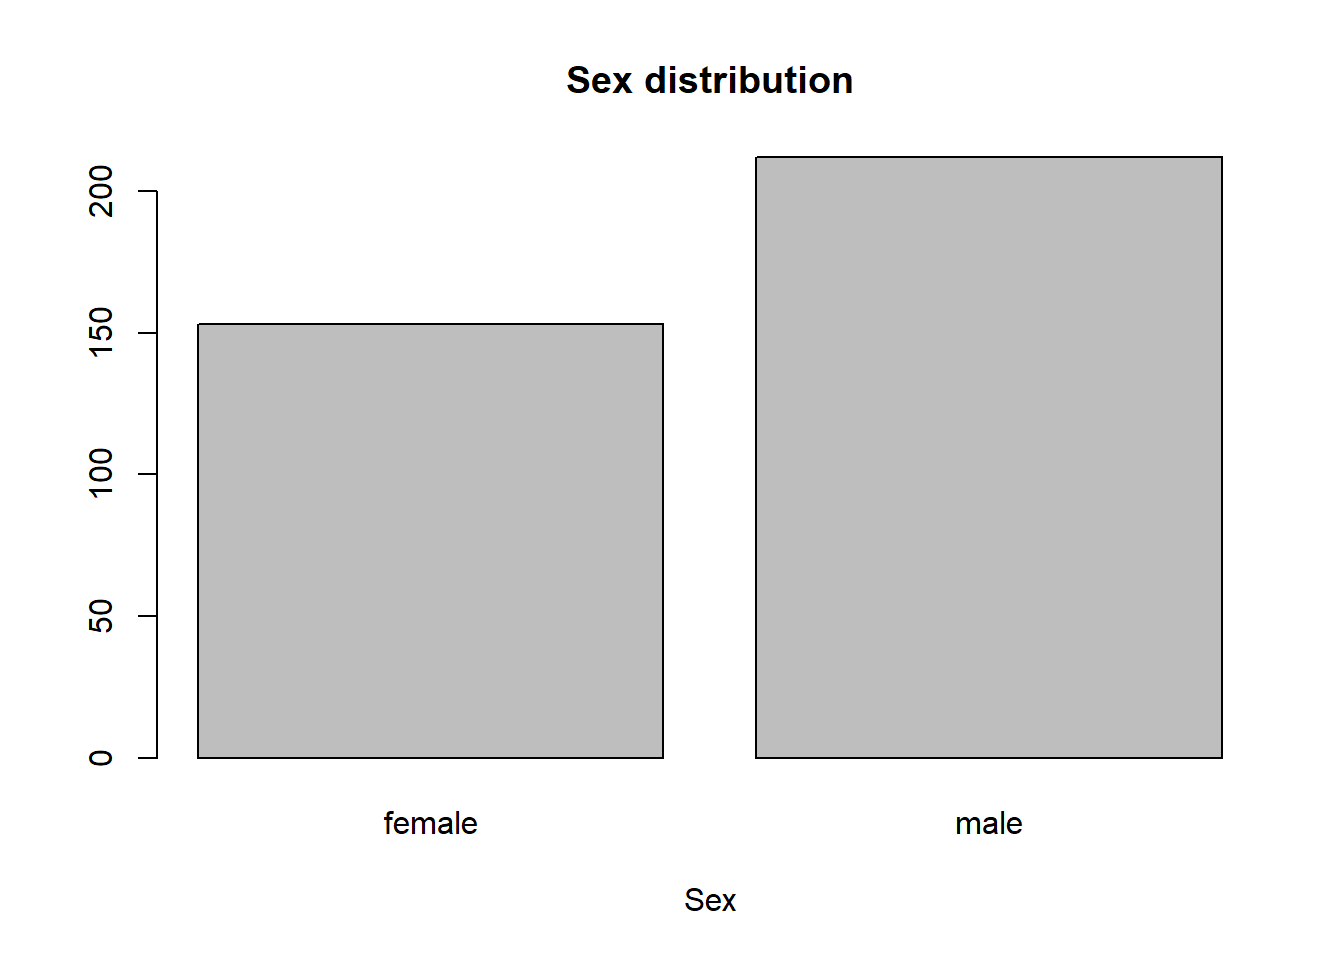
\includegraphics{bookdown-demo_files/figure-latex/unnamed-chunk-57-1.pdf}

\subsection{One variable: A numerical
variable}\label{one-variable-a-numerical-variable}

histogram

\begin{Shaded}
\begin{Highlighting}[]
\KeywordTok{hist}\NormalTok{(dataSPSS}\OperatorTok{$}\NormalTok{age, }\DataTypeTok{main =} \StringTok{'Age'}\NormalTok{,}
     \DataTypeTok{xlab=}\StringTok{'Age in years'}\NormalTok{,}
     \DataTypeTok{ylab=}\StringTok{'Count'}\NormalTok{)}
\end{Highlighting}
\end{Shaded}

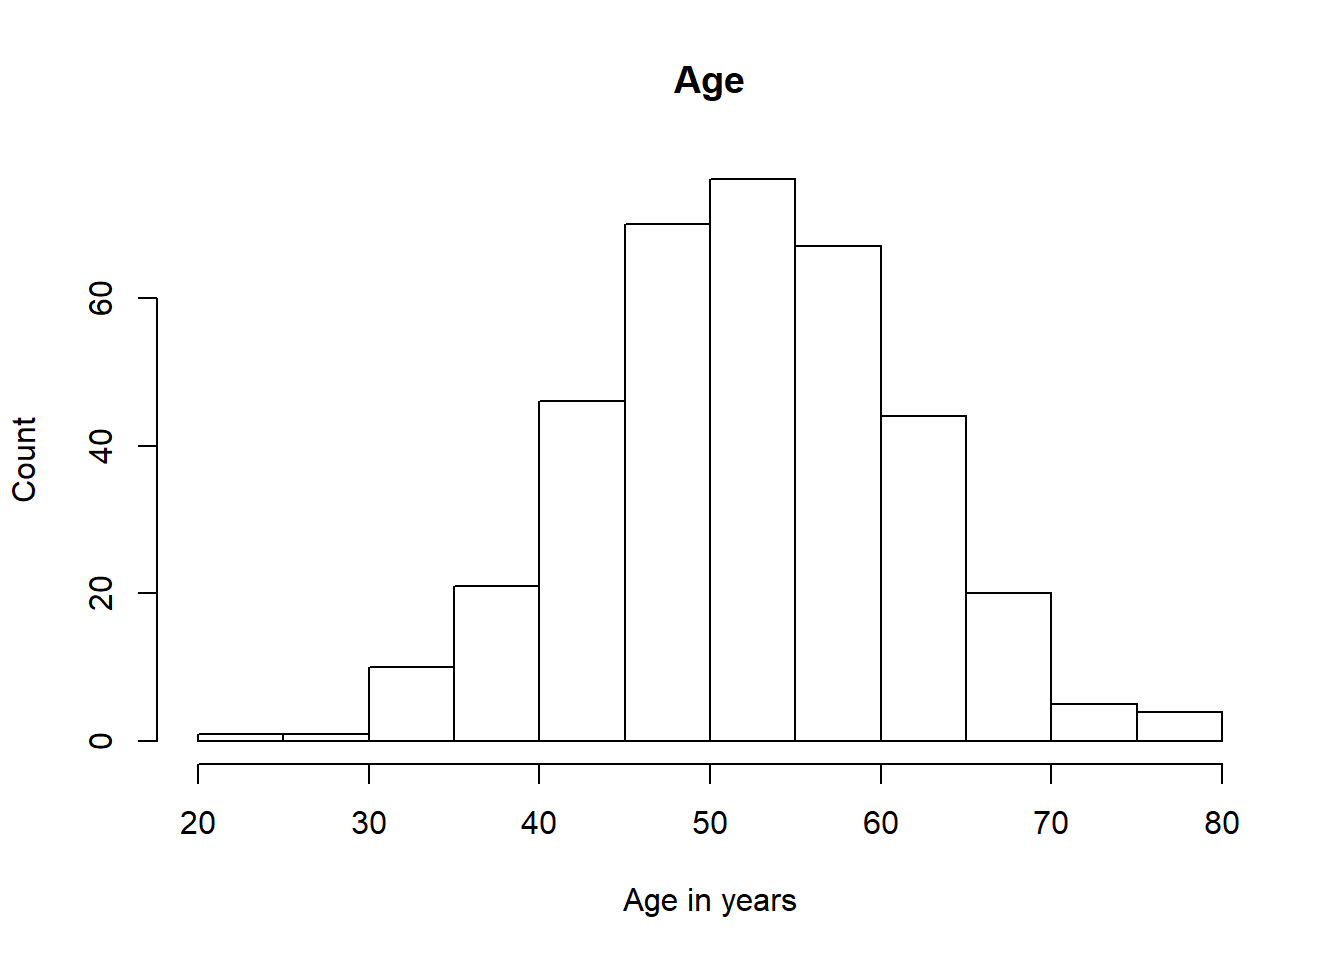
\includegraphics{bookdown-demo_files/figure-latex/unnamed-chunk-58-1.pdf}

\subsection{Two variables : A numerical with another numerical
variable}\label{two-variables-a-numerical-with-another-numerical-variable}

We will use \emph{scatterplot} to plot

\begin{Shaded}
\begin{Highlighting}[]
\KeywordTok{plot}\NormalTok{(dataSPSS}\OperatorTok{$}\NormalTok{tahundx, dataSPSS}\OperatorTok{$}\NormalTok{age,}
     \DataTypeTok{main =} \StringTok{'Duration having DM VS age'}\NormalTok{,}
     \DataTypeTok{xlab =} \StringTok{'Duration of DM'}\NormalTok{, }\DataTypeTok{ylab =} \StringTok{'Age'}\NormalTok{,}
     \DataTypeTok{pch =} \DecValTok{19}\NormalTok{)}
\end{Highlighting}
\end{Shaded}

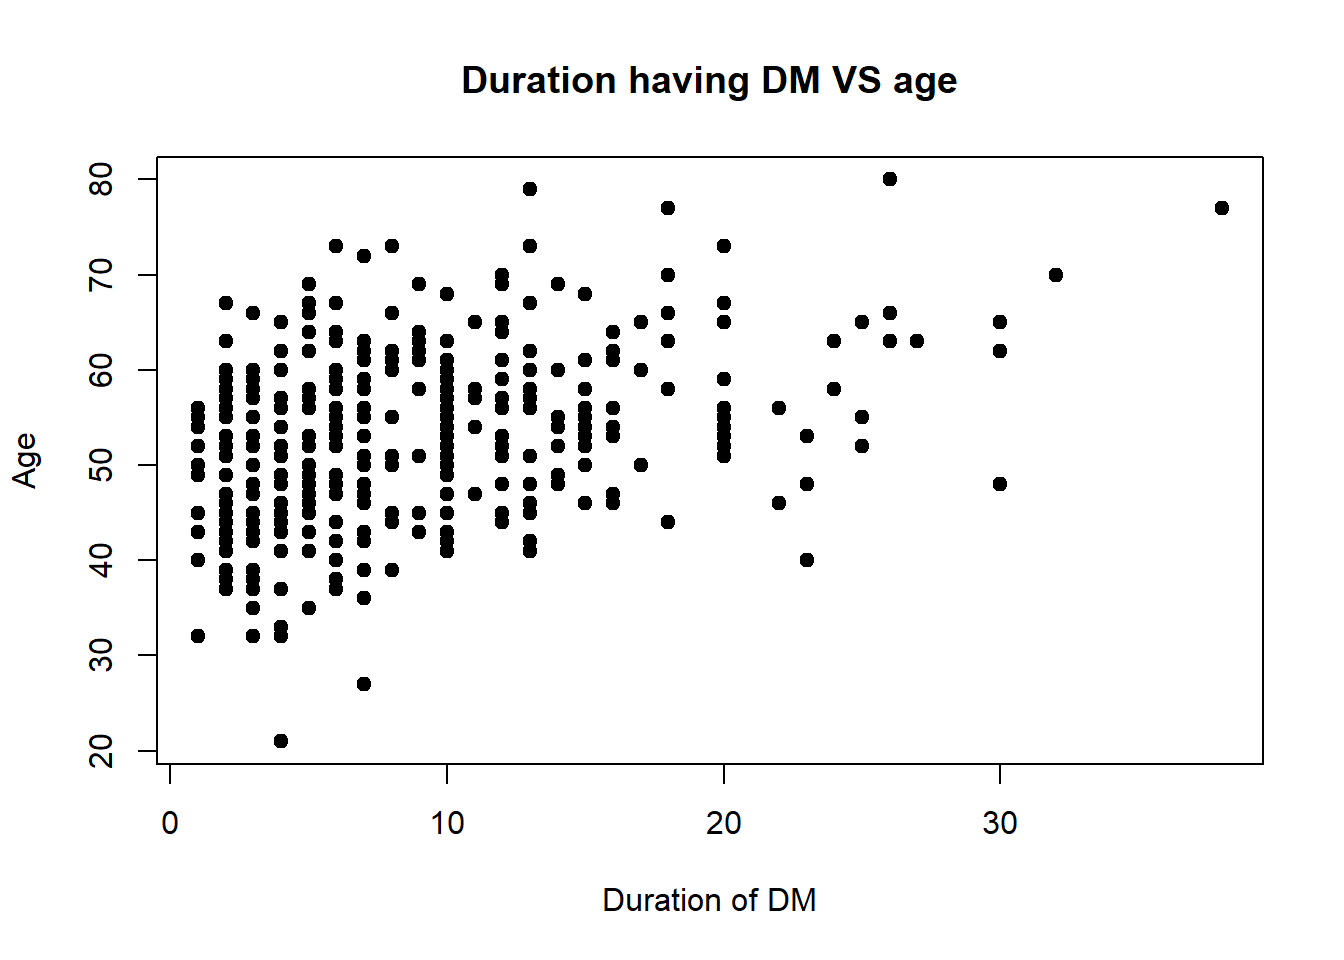
\includegraphics{bookdown-demo_files/figure-latex/unnamed-chunk-59-1.pdf}

Let us make a fit line

\begin{Shaded}
\begin{Highlighting}[]
\KeywordTok{plot}\NormalTok{(dataSPSS}\OperatorTok{$}\NormalTok{tahundx, dataSPSS}\OperatorTok{$}\NormalTok{age,}
     \DataTypeTok{main =} \StringTok{'Duration having DM VS age'}\NormalTok{,}
     \DataTypeTok{xlab =} \StringTok{'Duration of DM'}\NormalTok{, }\DataTypeTok{ylab =} \StringTok{'Age'}\NormalTok{,}
     \DataTypeTok{pch =} \DecValTok{19}\NormalTok{)}
\KeywordTok{abline}\NormalTok{(}\KeywordTok{lm}\NormalTok{(dataSPSS}\OperatorTok{$}\NormalTok{age}\OperatorTok{~}\NormalTok{dataSPSS}\OperatorTok{$}\NormalTok{tahundx), }\DataTypeTok{col =} \StringTok{'red'}\NormalTok{)}
\end{Highlighting}
\end{Shaded}

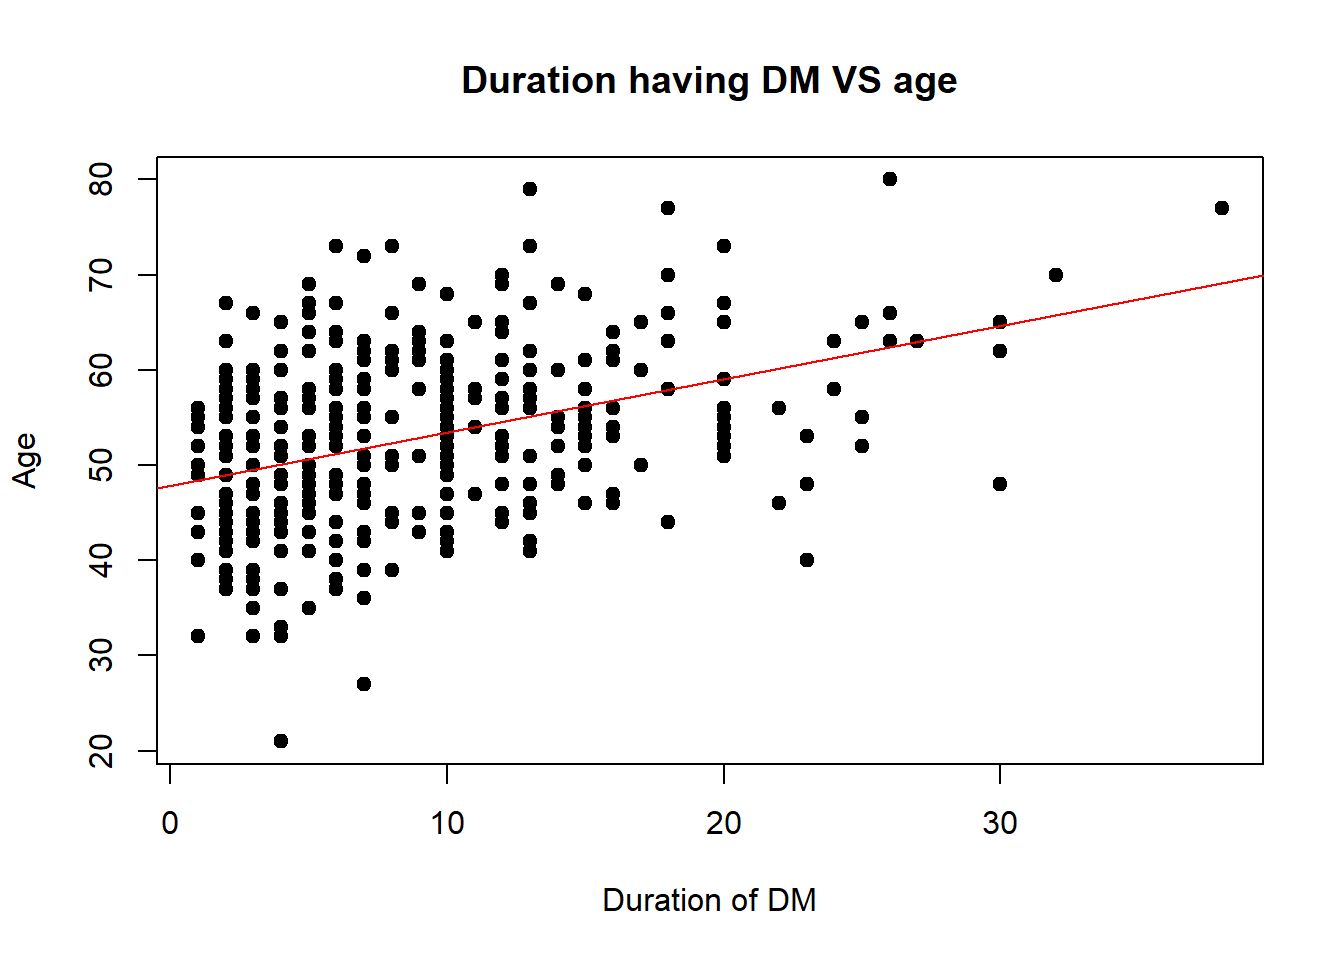
\includegraphics{bookdown-demo_files/figure-latex/unnamed-chunk-60-1.pdf}

and a lowess

\begin{Shaded}
\begin{Highlighting}[]
\KeywordTok{plot}\NormalTok{(dataSPSS}\OperatorTok{$}\NormalTok{tahundx, dataSPSS}\OperatorTok{$}\NormalTok{age,}
     \DataTypeTok{main =} \StringTok{'Duration having DM VS age'}\NormalTok{,}
     \DataTypeTok{xlab =} \StringTok{'Duration of DM'}\NormalTok{, }\DataTypeTok{ylab =} \StringTok{'Age'}\NormalTok{,}
     \DataTypeTok{pch =} \DecValTok{19}\NormalTok{)}
\KeywordTok{lines}\NormalTok{(}\KeywordTok{lowess}\NormalTok{(dataSPSS}\OperatorTok{$}\NormalTok{tahundx,dataSPSS}\OperatorTok{$}\NormalTok{age), }\DataTypeTok{col =} \StringTok{'blue'}\NormalTok{)}
\end{Highlighting}
\end{Shaded}

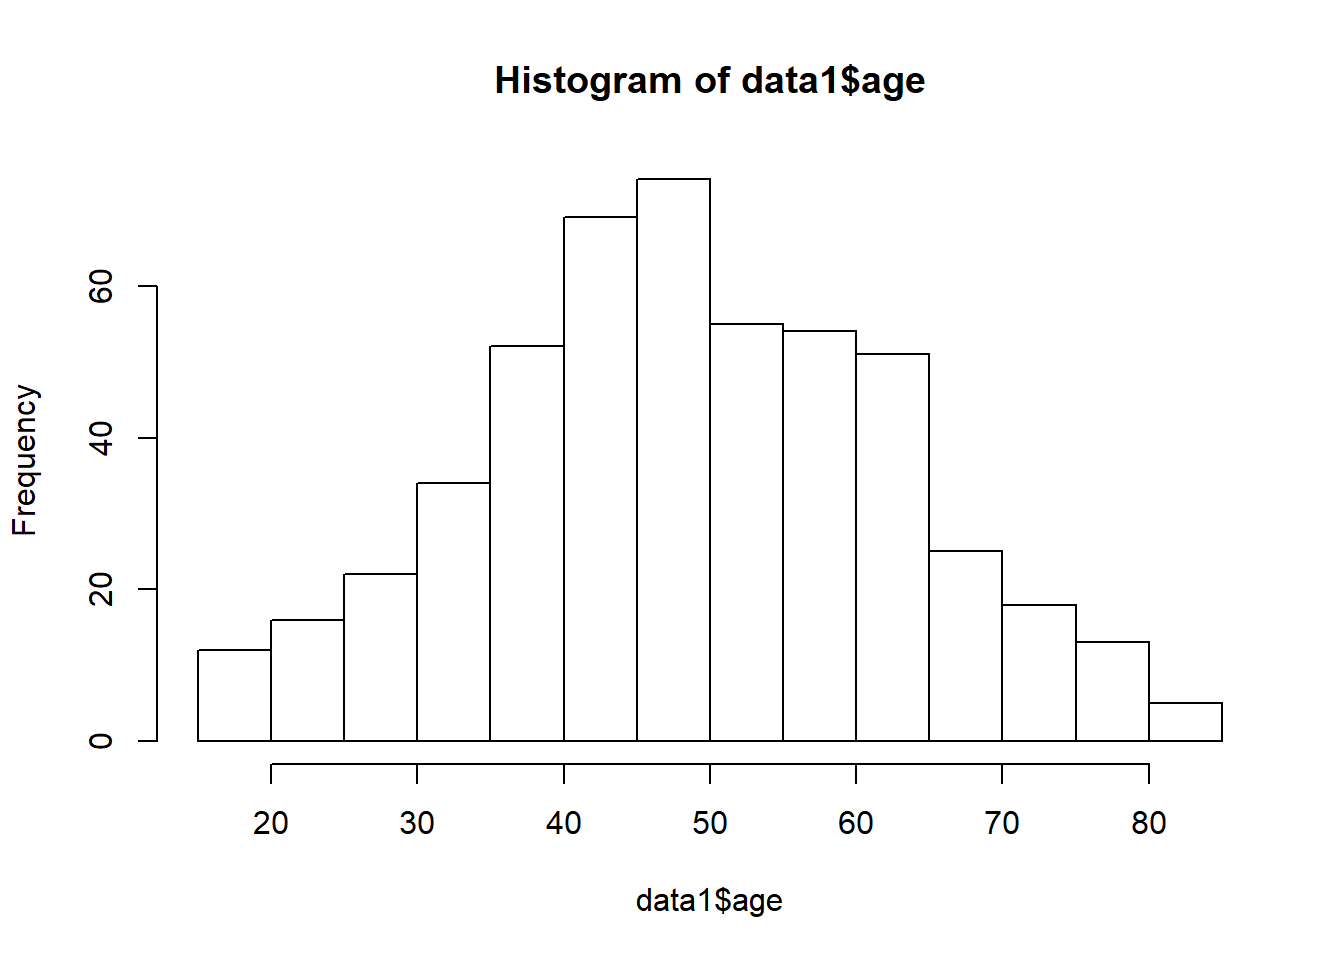
\includegraphics{bookdown-demo_files/figure-latex/unnamed-chunk-61-1.pdf}

\subsection{Two variables : A categorical variable with a categorical
variable}\label{two-variables-a-categorical-variable-with-a-categorical-variable}

Now, we will plot 2 categorical variables simultenously.

First, we will use stacked barchart

\begin{Shaded}
\begin{Highlighting}[]
\NormalTok{compl.sex<-}\KeywordTok{table}\NormalTok{(dataSPSS}\OperatorTok{$}\NormalTok{complica,dataSPSS}\OperatorTok{$}\NormalTok{sex)}
\NormalTok{compl.sex}
\end{Highlighting}
\end{Shaded}

\begin{verbatim}
##      
##       female male
##   no     105  120
##   yes     48   92
\end{verbatim}

\begin{Shaded}
\begin{Highlighting}[]
\KeywordTok{barplot}\NormalTok{(compl.sex,}
        \DataTypeTok{main=}\StringTok{'Complications by sex'}\NormalTok{,}
        \DataTypeTok{xlab=}\StringTok{'Sex'}\NormalTok{,}
        \DataTypeTok{col=}\KeywordTok{c}\NormalTok{(}\StringTok{'blue'}\NormalTok{,}\StringTok{'red'}\NormalTok{),}
        \DataTypeTok{legend=}\KeywordTok{c}\NormalTok{(}\StringTok{'No'}\NormalTok{,}\StringTok{'Yes'}\NormalTok{))}
\end{Highlighting}
\end{Shaded}

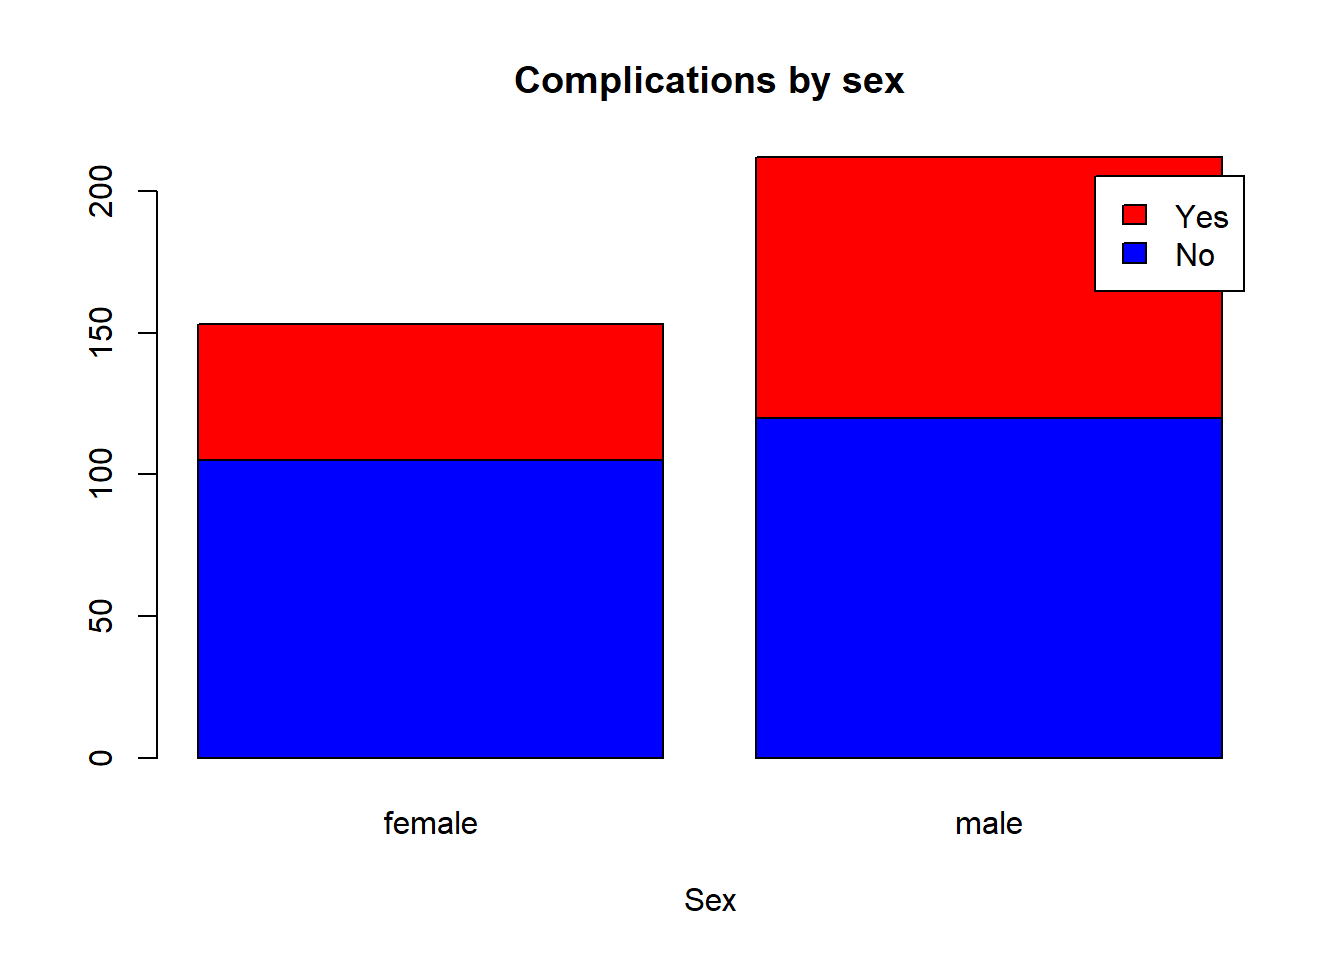
\includegraphics{bookdown-demo_files/figure-latex/unnamed-chunk-62-1.pdf}

Next, we will use grouped barchart

\begin{Shaded}
\begin{Highlighting}[]
\NormalTok{compl.sex}
\end{Highlighting}
\end{Shaded}

\begin{verbatim}
##      
##       female male
##   no     105  120
##   yes     48   92
\end{verbatim}

\begin{Shaded}
\begin{Highlighting}[]
\KeywordTok{barplot}\NormalTok{(compl.sex,}
        \DataTypeTok{main =} \StringTok{'Complications according to sex'}\NormalTok{,}
        \DataTypeTok{xlab =} \StringTok{'Sex'}\NormalTok{,}
        \DataTypeTok{col =} \KeywordTok{c}\NormalTok{(}\StringTok{'blue'}\NormalTok{,}\StringTok{'red'}\NormalTok{),}
        \DataTypeTok{legend =} \KeywordTok{c}\NormalTok{(}\StringTok{'no'}\NormalTok{,}\StringTok{'yes'}\NormalTok{),}
        \DataTypeTok{beside =} \OtherTok{TRUE}\NormalTok{)}
\end{Highlighting}
\end{Shaded}

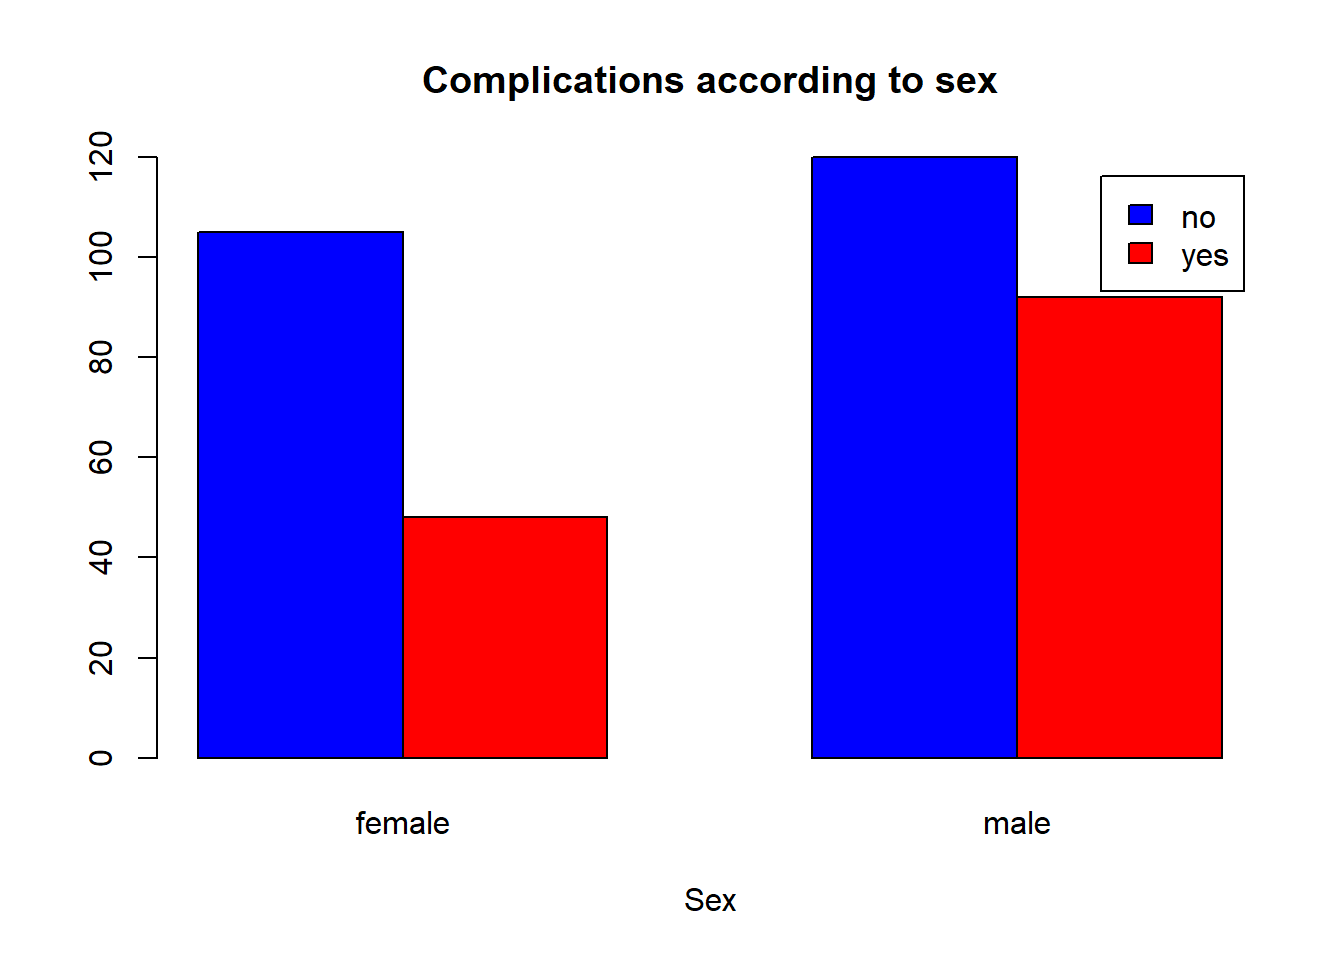
\includegraphics{bookdown-demo_files/figure-latex/unnamed-chunk-63-1.pdf}

\chapter{Graphical}\label{graphical}

Test GIT Test GIT 2 - commit

\chapter{Reporting results}\label{reporting-results}

\chapter{Final Words}\label{final-words}

We have finished a nice book.

\bibliography{packages,book}


\end{document}
